\chapter{Computational Paths}

\let\thefootnote\relax\footnote{This chapter is based on two papers published by the author (jointly with his advisor and co-advisor): \emph{Propositional equality, identity types, and computational paths} in \emph{South American Joournal of Logic}, 2016 \cite{Ruy1} and \emph{On the Identity Type as the Type of Computational Paths} in \emph{Logic Journal of the IGPL}, 2017 \cite{Art3}.}

In this chapter, we introduce the main concept of this work, an entity known as computational paths. In \textbf{chapter 2}, we have seen that it is possible to interpret the identity type semantically, considering the terms as homotopical paths between two points of a space. Nevertheless, there is no entity that represents those paths in the syntax of type theory. Thus, we add computational paths to fill this gap. In this sense, our objective is to formulate the identity type using this new entity.

This work has also been motivated by the fact that  although beautifully defined, we have noticed that proofs that uses the identity type can be sometimes a little too complex. The elimination rule of the intensional identity type encapsulates lots of information, sometimes making too troublesome the process of finding the reason that builds the correct type. We have also seen this in \textbf{chapter 2}. We proposed constructions for the symmetry and transitivity of the identity type. Although one could expect those constructions to be pretty straightforward, the process of obtaining the right reason to construct those types was troublesome.

Thus, inspired by the path-based approach of the homotopy interpretation, we believe that a similar approach can be used to define the identity type in type theory. To achieve that, we have been using a notion of {\em computational paths}. The interpretation will be similar to the homotopy one: a term $p : Id_{A}(a,b)$ will be a computational path between terms $a, b : A$, and such path will be the result of a sequence of rewrites. In the sequel, we shall define formally the concept of a computational path. The main idea, i.e.\ proofs of equality statements as (reversible) sequences of rewrites, is not new, as it goes back to a paper entitled ``Equality in labeled deductive systems and the functional interpretation of propositional equality ", presented in December 1993 at the {\em 9th Amsterdam Colloquium\/}, and published in the proceedings in 1994\cite{Ruy4}.

In the previous chapter, we have seen the concept of higher structures such as higher categories. Indeed, one of the most interesting aspects of the identity type is the fact that it can be used to construct higher structures. This is a rather natural consequence of the fact that it is possible to construct higher identities. For any $a, b : A$, we have type $Id_{A}(a,b)$. If this type is inhabited by any $p, q:Id_{A}(a,b)$, then we have type $Id_{Id_{A}(a,b)}(p,q)$. If the latter type is inhabited, we have a higher equality between $p$ and $q$\cite{harper1}. This concept is also present in computational paths. One can show the equality between two computational paths $s$ and $t$ by constructing a third one between $s$ and $t$. We show in this chapter a system of rules used to establish equalities between computational paths\cite{Anjo1}. Then, we show that these higher equalities go up to the infinity, forming a $\infty$-globular-set. We also show that computational paths naturally induce a groupoid structure. We also go a step further, showing that computational paths are capable of inducing a higher groupoid structure.

Another important question we want to answer is one that arises naturally when talking about equality: Is there a canonical proof for an expression $t_{1} = t_{2}$? In the language of computational paths, is there a normal path between $t_{1} = t_{2}$ such that every other path can be reduced to this one? In fact, we are going to prove that the answer is negative. Our model also refute the \gls{uip}).


\section{Introducing Computational Paths} \label{path}

Before we enter in details of computational paths, let's recall what motivated the introduction of computational paths to type theory. In type theory, our types are interpreted using the so-called Brower-Heyting-Kolmogorov Interpretation. That way, a semantic interpretation of types are not given by truth-values, but by the concept of proof as a primitive notion. Thus, we have \cite{Ruy1}:

\begin{tabbing}
	\textbf{a proof of the proposition:} \hbox{\ \ \ \ \ } \= \textbf{is given by:} \\
	$A\land B$ \> a proof of $A$ \textbf{and} a proof of $B$ \\ 
	$A\lor B$ \> a proof of $A$ \textbf{or} a proof of $B$ \\
	$A\rightarrow B$ \> a \textbf{function} that turns a proof of $A$ into a proof of $B$ \\
	$\forall x^D.P(x)$ \> a \textbf{function} that turns an element $a$ into a proof of $P(a)$ \\
	$\exists x^D.P(x)$ \> an element $a$ (witness) \textbf{and a proof of} $P(a)$ \\
\end{tabbing}

Also, based on the Curry-Howard functional interpretation of logical connectives, one have \cite{Ruy1}:

\begin{tabbing}
	\textbf{a proof of the proposition:} \hbox{\ \ \ \ \ } \= \textbf{has the canonical form of:} \\
	$A\land B$ \> $\langle p,q\rangle$ where $p$ is a proof of $A$ and $q$ is a proof of $B$ \\
	$A\lor B$ \> $i(p)$ where $p$ is a proof of $A$ or $j(q)$ where $q$ is a proof of $B$ \\
	\> (`$i$' and `$j$' abbreviate `into the left/right disjunct') \\
	$A\rightarrow B$ \> $\lambda x.b(x)$ where $b(p)$ is a proof of B \\
	\> provided $p$ is a proof of A \\
	$\forall x^A.B(x)$ \> $\Lambda x.f(x)$ where $f(a)$ is a proof of $B(a)$ \\ 
	\> provided $a$ is an arbitrary individual chosen\\
	\> from the domain $A$\\ 
	$\exists x^A.B(x)$ \> $\varepsilon x.(f(x),a)$ where $a$ is a witness\\
	\> from the domain $A$, $f(a)$ is a proof of $B(a)$ \\
\end{tabbing}

If one looks closely, there is one interpretation missing in the BHK-Interpretation. What constitutes a proof of $t_{1} = t_{2}$? In other words, what is a proof of an equality statement? We answer this by proposing that an equality between those two terms should be a sequence of rewrites starting from $t_{1}$ and ending at $t_{2}$. Thus, we would have \cite{Ruy1}:

\begin{tabbing}
	\textbf{a proof of the proposition:} \hbox{\ \ \ \ \ } \= \textbf{is given by:} \\
	\\
	$t_1= t_2$ \> ? \\
	\> (Perhaps a sequence of rewrites \\
	\> starting from $t_1$ and ending in $t_2$?) \\
\end{tabbing}

We call computational path the sequence of rewrites between these terms.

\subsection{Formal Definition}

Since computational path is a generic term, it is important to emphasize the fact that we are using the term computational path in the sense defined by\cite{Ruy5}. A computational path is based on the idea that it is possible to formally define when two computational objects $a,b : A$ are equal. These two objects are equal if one can reach $b$ from $a$ by applying a sequence of axioms or rules. This sequence of operations forms a path. Since it is between two computational objects, it is said that this path is a computational one. Also, an application of an axiom or a rule transforms (or rewrite) an term in another. For that reason, a computational path is also known as a sequence of rewrites. Nevertheless, before we define formally a computational path, we can take a look at one famous equality theory, the $\lambda\beta\eta-equality$\cite{lambda}:

\begin{mydefi}
	The \emph{$\lambda\beta\eta$-equality} is composed by the following axioms:
	
	\begin{enumerate}
		\item[$(\alpha)$] $\lambda x.M = \lambda y.M[y/x]$ \quad if $y \notin FV(M)$;
		\item[$(\beta)$] $(\lambda x.M)N = M[N/x]$;
		\item[$(\rho)$] $M = M$;
		\item[$(\eta)$] $(\lambda x.Mx) = M$ \quad $(x \notin FV(M))$.
	\end{enumerate}
	
	And the following rules of inference:
	
	
	\bigskip
	\noindent
	\begin{bprooftree}
		\AxiomC{$M = M'$ }
		\LeftLabel{$(\mu)$ \quad}
		\UnaryInfC{$NM = NM'$}
	\end{bprooftree}
	\begin{bprooftree}
		\AxiomC{$M = N$}
		\AxiomC{$N = P$}
		\LeftLabel{$(\tau)$}
		\BinaryInfC{$M = P$}
	\end{bprooftree}
	
	\bigskip
	\noindent
	\begin{bprooftree}
		\AxiomC{$M = M'$ }
		\LeftLabel{$(\nu)$ \quad}
		\UnaryInfC{$MN = M'N$}
	\end{bprooftree}
	\begin{bprooftree}
		\AxiomC{$M = N$}
		\LeftLabel{$(\sigma)$}
		\UnaryInfC{$N = M$}
	\end{bprooftree}
	
	\bigskip
	\noindent
	\begin{bprooftree}
		\AxiomC{$M = M'$ }
		\LeftLabel{$(\xi)$ \quad}
		\UnaryInfC{$\lambda x.M= \lambda x.M'$}
	\end{bprooftree}
	
	\bigskip
	%\bigskip
	%\noindent
	%\begin{bprooftree}
	%\AxiomC{$Mx = Nx$ }
	%\LeftLabel{$(\zeta)$ \quad}R
	%\UnaryInfC{$M = N$}R
	%\end{bprooftree}
	
	%\bigskip
	
	%If $M = N$ is provable in $\lambda\beta\eta$, then we say that  $\lambda\beta\eta \vdash M = N$.
	
\end{mydefi}

%Then, we can define the following equality relation \cite{lambda}:

%\begin{mydefi}
%The equality relation defined by $\lambda\beta\eta$-equality is called $=_{\beta\eta}$. In other words:

%\begin{center}
%$M =_{\beta\eta} N \Leftrightarrow \lambda\beta\eta \vdash M = N$.
%\end{center}

%\end{mydefi}

\begin{mydefi}\cite{lambda}
	$P$ is $\beta$-equal or $\beta$-convertible to $Q$  (notation $P=_\beta Q$)
	iff $Q$ is obtained from $P$ by a finite (perhaps empty)  series of $\beta$-contractions
	and reversed $\beta$-contractions  and changes of bound variables.  That is,
	$P=_\beta Q$ iff \textbf{there exist} $P_0, \ldots, P_n$ ($n\geq 0$)  such that
	$P_0\equiv P$,  $P_n\equiv Q$,
	$(\forall i\leq n-1) (P_i\triangleright_{1\beta}P_{i+1}  \mbox{ or }P_{i+1}\triangleright_{1\beta}P_i  \mbox{ or } P_i\equiv_\alpha P_{i+1}).$
\end{mydefi}
\noindent (Note that equality has an \textbf{existential} force, which will show in the proof rules for the identity type.)


The same happens with $\lambda\beta\eta$-equality:\\
\begin{mydefi}($\lambda\beta\eta$-equality\cite{lambda})
	The equality-relation determined by the theory $\lambda\beta\eta$ is called
	$=_{\beta\eta}$; that is, we define
	$$M=_{\beta\eta}N\quad\Leftrightarrow\quad\lambda\beta\eta\vdash M=N.$$
\end{mydefi}

\begin{example}
	Take the term $M\equiv(\lambda x.(\lambda y.yx)(\lambda w.zw))v$. Then, it is $\beta\eta$-equal to $N\equiv zv$ because of the sequence:\\
	$(\lambda x.(\lambda y.yx)(\lambda w.zw))v, \quad  (\lambda x.(\lambda y.yx)z)v, \quad   (\lambda y.yv)z , \quad zv$\\
	which starts from $M$ and ends with $N$, and each member of the sequence is obtained via 1-step $\beta$- or $\eta$-contraction of a previous term in the sequence. To take this sequence into a {\em path\/}, one has to apply transitivity twice, as we do in the example below.
\end{example}

\begin{example}\label{examplepath}
	The term $M\equiv(\lambda x.(\lambda y.yx)(\lambda w.zw))v$ is $\beta\eta$-equal to $N\equiv zv$ because of the sequence:\\
	$(\lambda x.(\lambda y.yx)(\lambda w.zw))v, \quad  (\lambda x.(\lambda y.yx)z)v, \quad   (\lambda y.yv)z , \quad zv$\\
	Now, taking this sequence into a path leads us to the following:\\
	The first is equal to the second based on the grounds:\\
	$\eta((\lambda x.(\lambda y.yx)(\lambda w.zw))v,(\lambda x.(\lambda y.yx)z)v)$\\
	The second is equal to the third based on the grounds:\\
	$\beta((\lambda x.(\lambda y.yx)z)v,(\lambda y.yv)z)$\\
	Now, the first is equal to the third based on the grounds:\\
	$\tau(\eta((\lambda x.(\lambda y.yx)(\lambda w.zw))v,(\lambda x.(\lambda y.yx)z)v),\beta((\lambda x.(\lambda y.yx)z)v,(\lambda y.yv)z))$\\
	Now, the third is equal to the fourth one based on the grounds:\\
	$\beta((\lambda y.yv)z,zv)$\\
	Thus, the first one is equal to the fourth one based on the grounds:\\
	$\tau(\tau(\eta((\lambda x.(\lambda y.yx)(\lambda w.zw))v,(\lambda x.(\lambda y.yx)z)v),\beta((\lambda x.(\lambda y.yx)z)v,(\lambda y.yv)z)),\beta((\lambda y.yv)z,zv)))$.
\end{example}

%Note again that two terms are $\lambda\beta\eta$-equal if {\bf there exists} a sequence of applications of rules of %definitional equality which builds
%a proof of their equality in the theory of $\lambda\beta\eta$-equality.

The aforementioned theory establishes the equality between two $\lambda$-terms. Since we are working with computational objects as terms of a type, we need to translate the $\lambda\beta\eta$-equality to a suitable equality theory based on Martin L\"of's type theory. We obtain:

\begin{mydefi}
	The equality theory of Martin L\"of's type theory has the following basic proof rules for the $\Pi$-type:
	
	\bigskip
	
	\noindent
	\begin{bprooftree}
		\hskip -0.3pt
		\alwaysNoLine
		\AxiomC{$N : A$}
		\AxiomC{$[x : A]$}
		\UnaryInfC{$M : B$}
		\alwaysSingleLine
		\LeftLabel{$(\beta$) \quad}
		\BinaryInfC{$(\lambda x.M)N = M[N/x] : B[N/x]$}
	\end{bprooftree}
	\begin{bprooftree}
		\hskip 11pt
		\alwaysNoLine
		\AxiomC{$[x : A]$}
		\UnaryInfC{$M = M' : B$}
		\alwaysSingleLine
		\LeftLabel{$(\xi)$ \quad}
		\UnaryInfC{$\lambda x.M = \lambda x.M' : (\Pi x : A)B$}
	\end{bprooftree}
	
	\bigskip
	
	\noindent
	\begin{bprooftree}
		\hskip -0.5pt
		\AxiomC{$M : A$}
		\LeftLabel{$(\rho)$ \quad}
		\UnaryInfC{$M = M : A$}
	\end{bprooftree}
	\begin{bprooftree}
		\hskip 100pt
		\AxiomC{$M = M' : A$}
		\AxiomC{$N : (\Pi x : A)B$}
		\LeftLabel{$(\mu)$ \quad}
		\BinaryInfC{$NM = NM' : B[M/x]$}
	\end{bprooftree}
	
	\bigskip
	
	\noindent
	\begin{bprooftree}
		\hskip -0.5pt
		\AxiomC{$M = N : A$}
		\LeftLabel{$(\sigma) \quad$}
		\UnaryInfC{$N = M : A$}
	\end{bprooftree}
	\begin{bprooftree}
		\hskip 105pt
		\AxiomC{$N : A$}
		\AxiomC{$M = M' : (\Pi x : A)B$}
		\LeftLabel{$(\nu)$ \quad}
		\BinaryInfC{$MN = M'N : B[N/x]$}
	\end{bprooftree}
	
	\bigskip
	
	\noindent
	\begin{bprooftree}
		\hskip -0.5pt
		\AxiomC{$M = N : A$}
		\AxiomC{$N = P : A$}
		\LeftLabel{$(\tau)$ \quad}
		\BinaryInfC{$M = P : A$}
	\end{bprooftree}
	
	\bigskip
	
	\noindent
	\begin{bprooftree}
		\hskip -0.5pt
		\AxiomC{$M: (\Pi x : A)B$}
		\LeftLabel{$(\eta)$ \quad}
		\RightLabel {$(x \notin FV(M))$}
		\UnaryInfC{$(\lambda x.Mx) = M: (\Pi x : A)B$}
	\end{bprooftree}
	
	\bigskip
	
\end{mydefi}

We are finally able to formally define computational paths:

\begin{mydefi}
	Let $a$ and $b$ be elements of a type $A$. Then, a \emph{computational path} $s$ from $a$ to $b$ is a composition of rewrites (each rewrite is an application of the inference rules of the equality theory of type theory or is a change of bound variables). We denote that by $a =_{s} b$.
\end{mydefi}

As we have seen in \emph{example \ref{examplepath}}, composition of rewrites are applications of the rule $\tau$. Since change of bound variables is possible, each term is considered up to $\alpha$-equivalence.

\subsection{Equality Equations}

One can use the aforementioned axioms to show that computational paths establishes the three fundamental equations of equality: the reflexivity, symmetry and transitivity:

\bigskip

\begin{bprooftree}
\AxiomC{$a =_{t} b : A$}
\AxiomC{$b =_{u} c : A$}
\RightLabel{\textit{transitivity}}
\BinaryInfC{$a =_{\tau(t,u)} c : A$}
\end{bprooftree}
\begin{bprooftree}
\AxiomC{$a : A$}
\RightLabel{\textit{reflexivity}}
\UnaryInfC{$a =_{\rho} a : A$}
\end{bprooftree}

\bigskip
\begin{bprooftree}
\AxiomC{$a =_{t} b : A$}
\RightLabel{\textit{symmetry}}
\UnaryInfC{$b =_{\sigma(t)} a : A$}
\end{bprooftree}

\bigskip

\subsection{Identity Type}

We have said that it is possible to formulate the identity type using computational paths. As we have seen, the best way to define any formal entity of type theory is by a set of natural deductions rules. Thus, we define our path-based approach as the following set of rules: 

\begin{itemize}
	
	\item Formation and Introduction rules \cite{Ruy1,Art3}:
	
	\bigskip
	\begin{center}
		\begin{bprooftree}
			\AxiomC{$A$ type}
			\AxiomC{$a : A$}
			\AxiomC{$b : A$}
			\RightLabel{$Id - F$}
			\TrinaryInfC{$Id_{A}(a,b)$ type}
		\end{bprooftree}
	
	\bigskip
	
		\begin{bprooftree}
			\AxiomC{$a =_{s} b : A$}
			\RightLabel{$Id - I$}
			\UnaryInfC{$s(a,b) : Id_{A}(a,b)$}
		\end{bprooftree}
	\end{center}
	\bigskip
	
	One can notice that our formation rule is exactly equal to the traditional identity type. From terms $a, b : A$, one can form that is inhabited only if there is a proof of equality between those terms, i.e., $Id_{A}(a,b)$.
	
	The difference starts with the introduction rule. In our approach, one can notice that we do not use a reflexive constructor $r$. In other words, the reflexive path is not the main building block of our identity type. Instead, if we have a computational path $a =_{s} b : A$, we introduce $s(a,b)$ as a term of the identity type. That way, one should see $s(a,b)$ as a sequence of rewrites and substitutions (i.e., a computational path) which would have started from $a$ and arrived at $b$
	
	\bigskip 
	
	\item Elimination rule \cite{Ruy1,Art3}:
	
	\begin{center}
		\begin{bprooftree}
			\alwaysNoLine
			\AxiomC{$m : Id_{A}(a,b)$ }
			\AxiomC{$[a =_{g} b : A]$}
			\UnaryInfC{$h(g) : C$}
			\alwaysSingleLine
			\RightLabel{$Id - E$}
			\BinaryInfC{$REWR(m, \acute{g}.h(g)) : C$}
		\end{bprooftree}
	\end{center}
	\bigskip
	
	Let's recall the notation being used. First, one should see $h(g)$ as a functional expression $h$ which depends on $g$. Also, one should notice the use of `$\acute{\ }$' in $\acute{g}$. One should see `$\acute{\ }$' as an abstractor that binds the occurrences of the variable $g$ introduced in the local assumption $[a =_{g} b : A]$ as a kind of {\em Skolem-type\/} constant denoting the {\em reason\/} why $a$ was assumed to be equal to $b$.
	
	We also introduce the constructor $REWR$. In a sense, it is similar to the constructor $J$ of the traditional approach, since both arise from the elimination rule of the identity type. The behavior of $REWR$ is simple. If from a computational path $g$ that establishes the equality between $a$ and $b$ one can construct $h(g) : C$, then if we also have this equality established by a term $m : Id_{A}(a,b)$, we can put together all this information in $REWR$ to construct $C$, eliminating the type $Id_{A}(a,b)$ in the process. The idea is that we can substitute $g$ for $m$ in $\acute{g}.h(g)$, resulting in $h(m/g) : C$. This behavior is established next by the reduction rule.
	
	\item Reduction rule 	\cite{Ruy1,Art3}:
	
	\bigskip
	\begin{center}
		\begin{bprooftree}
			\AxiomC{$a =_{m} b : A$}
			\RightLabel{$Id - I$}
			\UnaryInfC{$m(a,b) : Id_{A}(a,b)$}
			\alwaysNoLine
			\AxiomC{$[a =_{g} b : A]$}
			\UnaryInfC{$h(g) : C$}
			\alwaysSingleLine
			\RightLabel{$Id - E$ \quad $\rhd_\beta$}
			\BinaryInfC{$REWR(m, \acute{g}.h(g)) : C$}
		\end{bprooftree}
		\begin{bprooftree}
			\AxiomC{$[a =_{m} b : A]$}
			\alwaysNoLine
			\UnaryInfC{$h(m/g):C$}
		\end{bprooftree}
	\end{center}
	\bigskip
	
	\item Induction rule:
	
	\bigskip
	\begin{center}
		\begin{bprooftree}
			\AxiomC{$e : Id_{A}(a,b)$}
			\AxiomC{$[a =_{t} b : A]$}
			\RightLabel{$Id - I$}
			\UnaryInfC{$t(a, b) : Id_{A}(a, b)$}
			\RightLabel{$Id - E$ \quad  $\rhd_{\eta}$ \quad $e : Id_{A}(a,b)$}
			\BinaryInfC{$REWR(e, \acute{t}.t(a,b)) : Id_{A}(a,b)$}
		\end{bprooftree}
	\end{center}
	\bigskip
	
\end{itemize}

Our introduction and elimination rules reassure the concept of equality as an \textbf{existential force}. In the introduction rule, we encapsulate the idea that a witness of a identity type $Id_{A}(a,b)$ only exists if there exist a computational path establishing the equality of $a$ and $b$. Also, one can notice that our elimination rule is similar to the elimination rule of the existential quantifier.

\subsection{Path-based Examples}

The objective of this subsection is to show how to use in practice the rules that we have just defined. The idea is to show construction of terms of some important types. The constructions that we have chosen to build are the reflexive, transitive and symmetric type of the identity type. Those were not random choices. The main reason is the fact that reflexive, transitive and symmetric types are essential to the process of building a groupoid model for the identity type\cite{hofmann1}. As we shall see, these constructions come naturally from simple computational paths constructed by the application of axioms of the equality of type theory.

Before we start the constructions, we think that it is essential to understand how to use the eliminations rules. The process of building a term of some type is a matter of finding the right reason. In the case of $J$, the reason is the correct $x,y : A$ and $z : Id_{A}(a,b)$ that generates the adequate $C(x,y,z)$. In our approach, the reason is the correct path $a =_{g} b$ that generates the adequate $g(a,b) : Id(a,b)$.


\subsubsection{Reflexivity}

One could find strange the fact that we need to prove the reflexivity. Nevertheless, just remember that our approach is not based on the idea that reflexivity is the base of the identity type. As usual in type theory, a proof of something comes down to a construction of a term of a type. In this case, we need to construct a term of type $\Pi_{(a : A)}Id_{A}(a,a)$. The reason is extremely simple: from a term $a : A$, we obtain the computational path $a =_{\rho} a : A$ \cite{Art3}:

\bigskip

\begin{center}
	\begin{bprooftree}
		\AxiomC{$[a : A]$}
		\UnaryInfC{$a =_{\rho} a : A$}
		\RightLabel{$Id - I$}
		\UnaryInfC{$\rho(a,a) : Id_{A}(a,a)$}
		\RightLabel{$\Pi-I$}
		\UnaryInfC{$\lambda a.\rho(a,a) : \Pi_{(a : A)}Id_{A}(a,a)$}
	\end{bprooftree}
\end{center}

\bigskip

\subsubsection{Symmetry}

The second proposed construction is the symmetry. Our objective is to obtain a term of type  $\Pi_{(a : A)}\Pi_{(b : A)}(Id_{A}(a,b) \rightarrow Id_{A}(b,a))$.

We construct a proof using computational paths. As expected, we need to find a suitable reason. Starting from $a =_{t} b$, we could look at the axioms of \emph{definition 4.1} to plan our next step. One of those axioms makes the symmetry clear: the $\sigma$ axiom. If we apply $\sigma$, we will obtain $b =_{\sigma(t)} a$. From this, we can then infer that $Id_A$ is inhabited by $(\sigma(t))(b,a)$. Now, it is just a matter of applying the elimination \cite{Art3}:

\bigskip

\begin{center}
	\begin{bprooftree}
		\alwaysNoLine
		\AxiomC{$[a:A] \quad [b:A]$}
		\UnaryInfC{$[p(a,b) : Id_{A}(a,b)]$}
		\alwaysSingleLine
		\AxiomC{[$a =_{t} b : A$]}
		\UnaryInfC{$b =_{\sigma(t)} a : A$}
		\RightLabel{$Id - I$}
		\UnaryInfC{$(\sigma(t))(b,a) : Id_{A}(b,a)$}
		\RightLabel{$Id - E$}
		\BinaryInfC{$REWR(p(a,b),\acute{t}.(\sigma(t))(b,a)) : Id_{A}(b,a)$}
		\RightLabel{$\rightarrow - I$}
		\UnaryInfC{$\lambda p.REWR(p(a,b), \acute{t}.(\sigma(t))(b,a)) : Id_{A} (a,b) \rightarrow Id_{A}(b,a)$}
		\RightLabel{$\Pi-I$}
		\UnaryInfC{$\lambda b. \lambda p.REWR(p(a,b),\acute{t}.(\sigma(t))(b,a)) :  \Pi_{(b : A)}(Id_{A} (a,b) \rightarrow Id_{A}(b,a))$}
		\RightLabel{$\Pi-I$}
		\UnaryInfC{$\lambda a.\lambda b. \lambda p.REWR(p(a,b), \acute{t}.(\sigma(t))(b,a)) :  \Pi_{(a : A)}\Pi_{(b : A)}(Id_{A} (a,b) \rightarrow Id_{A}(b,a))$}
	\end{bprooftree}
\end{center}

\bigskip

\subsubsection{Transitivity}
The third and last construction will be the transitivity. Our objective os to obtain a term of type  $\Pi_{(a : A)}\Pi_{(b : A)}\Pi_{(c : A)} (Id_{A}(a,b) \rightarrow Id_{A}(b,c) \rightarrow Id_{A}(a,c))$.

To build our path-based construction, the first step, as expected, is to find the reason. Since we are trying to construct the transitivity, it is natural to think that we should start with paths $a =_{t} b$ and $b =_{u} c$ and then, from these paths, we should conclude that there is a path $z$ that establishes that $a =_{z} c$. To obtain $z$, we could try to apply the axioms of \emph{definition 4.1}. Looking at the axioms, one is exactly what we want: the axiom $\tau$. If we apply $\tau$ to  $a =_{t} b$ and $b =_{u} c$, we will obtain a new path $\tau(t,u)$ such that $a = _{\tau(t,u)} c$. Using that construction as the reason, we obtain the following term \cite{Art3}:

\begin{center}
	\begin{figure}
		\begin{sideways}
		\begin{bprooftree}
			\alwaysNoLine
			\AxiomC{$[a:A] \quad [b:A]$}
			\UnaryInfC{$[w(a,b) : Id_{A}(a,b)]$}
			\alwaysNoLine
			\AxiomC{$[c:A]$}
			\UnaryInfC{$[s(b,c) : Id_{A}(b,c)]$}
			\alwaysSingleLine
			\AxiomC{$[a =_{t} b:A]$}
			\AxiomC{$[b =_{u} c:A]$}
			\BinaryInfC{$a =_{\tau(t,u)} c:A$}
			\RightLabel{$Id - I$}
			\UnaryInfC{$(\tau (t,u))(a,c) : Id_{A}(a,c)$}
			\RightLabel{$Id - E$}
			\BinaryInfC{$REWR(s(b,c),\acute{u}(\tau (t,u))(a,c)) : Id_{A}(a,c)$}
			\RightLabel{$Id - E$}
			\BinaryInfC{$REWR(w(a,b),\acute{t}REWR(s(b,c),\acute{u}(\tau (t,u))(a,c))) : Id_{A}(a,c)$}
			\RightLabel{$\rightarrow - I$}
			\UnaryInfC{$\lambda s.REWR(w(a,b),\acute{t}REWR(s(b,c),\acute{u}(\tau (t,u))(a,c))) : Id_{A}(b,c) \rightarrow Id_{A}(a,c)$}
			\RightLabel{$\rightarrow - I$}
			\UnaryInfC{$\lambda w.\lambda s.REWR(w(a,b),\acute{t}REWR(s(b,c),\acute{u}(\tau (t,u))(a,c))) : Id_{A}(a,b) \rightarrow Id_{A}(b,c) \rightarrow Id_{A}(a,c)$}
			\RightLabel{$\Pi-I$}
			\UnaryInfC{$\lambda c.\lambda w.\lambda s.REWR(w(a,b),\acute{t}REWR(s(b,c),\acute{u}(\tau (t,u))(a,c))) :  \Pi_{(c : A)}(Id_{A}(a,b) \rightarrow Id_{A}(b,c) \rightarrow Id_{A}(a,c))$}
			\RightLabel{$\Pi-I$}
			\UnaryInfC{$\lambda b. \lambda c.\lambda w.\lambda s.REWR(w(a,b),\acute{t}REWR(s(b,c),\acute{u}(\tau (t,u))(a,c))) :  \Pi_{(b : A)}\Pi_{(c : A)}(Id_{A}(a,b) \rightarrow Id_{A}(b,c) \rightarrow Id_{A}(a,c))$}
			\RightLabel{$\Pi-I$}
			\UnaryInfC{$\lambda a. \lambda b. \lambda c.\lambda w.\lambda s.REWR(w(a,b),\acute{t}REWR(s(b,c),\acute{u}(\tau (t,u))(a,c))) :   \Pi_{(a : A)}\Pi_{(b : A)}\Pi_{(c : A)}(Id_{A}(a,b) \rightarrow Id_{A}(b,c) \rightarrow Id_{A}(a,c))$}
		\end{bprooftree}
	\end{sideways}
	\end{figure}
	\end{center}


\newpage

As one can see, each step is just straightforward applications of introduction, elimination rules and abstractions. The only idea behind this construction is just the simple fact that the axiom $\tau$ guarantees the transitivity of paths. If one compares the reason of this construction to the one that used $J$ (we showed those constructions in chapter 2), one can clearly conclude that the reason of the path-based approach was obtained more naturally.

\section{Term Rewrite System}

As we have just shown, a computational path establishes when two terms of the same type are equal. From the theory of computational paths, an interesting case arises. Suppose we have a path $s$ that establishes that $a =_{s} b : A$ and a path $t$ that establishes that $a =_{t} b : A$. Consider that $s$ and $t$ are formed by distinct compositions of rewrites. Is it possible to conclude that there are cases that $s$ and $t$ should be considered equivalent? The answer is \emph{yes}. Consider the following examples \cite{ArtMestrado}:

\begin{example}
	\noindent \normalfont Consider the path  $a =_{t} b : A$. By the symmetric property, we obtain $b =_{\sigma(t)} a : A$. What if we apply the property again on the path $\sigma(t)$? We would obtain a path  $a =_{\sigma(\sigma(t))} b : A$. Since we applied symmetry twice in succession, we obtained a path that is equivalent to the initial path $t$. For that reason, we conclude the act of applying symmetry twice in succession is a redundancy. We say that the path $\sigma(\sigma(t))$ should be reduced to the path $t$.
\end{example}

\begin{example}

	\noindent \normalfont Consider the reflexive path $a =_{\rho} a : A$. It one applies the symmetric axiom, one ends up with $a =_{\sigma(\rho)} a : A$. Thus, the obtained path is equivalent to the initial one, since the symmetry was applied to the reflexive path. Therefore, $\sigma(\rho)$ is a redundant way of expressing the path $\rho$. Thus, $\sigma(\rho)$ should be reduced to $\rho$.
	
\end{example}

\begin{example}
	\noindent \normalfont Consider a path $a =_{t} b : A$. Applying the symmetry, one ends up with $b =_{\sigma(t)} a : A$. One can take those two paths and apply the transitivity, ending up with $a =_{\tau(t,\sigma(t))} a$. Since one path is the inverse of the other, the composition of those two paths should be equivalent to the reflexive path. Thus, $\tau(t,\sigma(t))$ should be reduced to $\rho$.
\end{example}	
	
As one could see in the aforementioned examples, different paths should be considered equal if one is just a redundant form of the other. The examples that we have just seen are just  straightforward and simple cases. Since the equality theory has a total of 7 axioms, the possibility of combinations that could generate redundancies are high. Fortunately, all possible redundancies were thoroughly mapped by\cite{Anjo1}. In that work, a system that establishes all redundancies and creates rules that solve them was proposed. This system, known as $LND_{EQ}-TRS$, maps a total of $39$ rules that solve redundancies. 

\subsection{$LND_{EQ}-TRS$}

In this subsection, we show the rules that compose the $LND_{EQ}-TRS$. All those rules comes from the mapping of redundancies between computational paths, as we have seen in the $3$ previous examples. 

\subsubsection{Subterm Substitution}

Before we introduce the rewriting rules, it is important to introduce the concept of subterm substitution. In Equational Logic, the subterm substitution is given by the following inference rule\cite{Ruy2}:
\begin{center}
	\begin{bprooftree}
		\AxiomC{$s = t$ }
		\UnaryInfC{$s\theta = t\theta$}
	\end{bprooftree}
\end{center}

One problem is that such rule does not respect the sub-formula property. To deal with that,\cite{Chenadec} proposes two inference rules:

\begin{center}
	\begin{bprooftree}
		\AxiomC{$M = N$}
		\AxiomC{$C[N] = O$}
		\RightLabel{$IL$ \quad}
		\BinaryInfC{$C[M] = O$}
	\end{bprooftree}
	\begin{bprooftree}
		\AxiomC{$M = C[N]$}
		\AxiomC{$N = O$}
		\RightLabel{$IR$ \quad}
		\BinaryInfC{$M = C[O]$}
	\end{bprooftree}
\end{center}

\noindent where M, N and O are terms.

As proposed in \cite{Ruy1}, we can define similar rules using computational paths, as follows:

\begin{center}
	\begin{bprooftree}
		\AxiomC{$x =_r {\cal C}[y]: A$}
		\AxiomC{$y =_s u : A'$}
		\BinaryInfC{$x =_{{\tt sub}_{\tt L}(r,s)} {\cal C}[u]: A$}
	\end{bprooftree}
	\begin{bprooftree}
		\AxiomC{$x =_r w : A'$}
		\AxiomC{${\cal C}[w]=_s u : A$}
		\BinaryInfC{${\cal C}[x]=_{{\tt sub}_{\tt R}(r,s)} u : A$}
	\end{bprooftree}
\end{center}

\noindent where $C$ is the context in which the sub-term detached by '[ ]' appears and $A'$ could be a sub-domain of $A$, equal to $A$ or disjoint to $A$.

In the rule above, ${\cal C}[u]$ should be understood as the result of replacing every occurrence of $y$ by $u$ in $C$.

\subsubsection{Rewriting Rules}

In this subsection, our objective is to show all rewrite reductions and their associated rewriting rules. The idea is to analyze all possible occurrences of redundancies in proofs which involves the rules of rewritings. 

We start with the transitivity:

\begin{mydefi}[reductions involving $\tau$ \cite{Ruy1}]
	
	\bigskip
	
	$$\displaystyle{ x =_r y : {A} \quad y =_{\sigma(r)} x :
		{A} \over x =_{\tau(r,\sigma(r))} x : {A}} \quad 
	\triangleright_{tr}  \quad x =_{\rho} x : {A}$$
	\bigskip
	$$\displaystyle{ y =_{\sigma (r)} x : {A} \quad x=_r y 
		:  {A} \over y =_{\tau(\sigma(r),r)} y : {A}} \quad \triangleright_{tsr} \quad  y=_{\rho} y : {A}$$
	\bigskip
	$$\displaystyle{ u=_r v : {A} \quad v=_{\rho} v :  
		{A} \over u =_{\tau(r,\rho)} v : {A}} \quad 
	\triangleright_{trr}  \quad  u =_r v : {A}$$
	\bigskip
	$$\displaystyle{ u=_{\rho} u : {A} \quad u=_r v : 
		{A} \over u=_{\tau(\rho, r)} v : {A}} \quad 
	\triangleright_{tlr}  \quad u=_r v : {A}$$
	\bigskip
	
	Associated rewriting rules:\\
	$\tau(r,\sigma(r))\triangleright_{tr}\rho$\\
	$\tau(\sigma(r),r) \triangleright_{tsr}\rho$\\
	$\tau(r,\rho) \triangleright_{trr} r$\\
	$\tau(\rho, r) \triangleright_{tlr} r$.\\
\end{mydefi} 

These reductions can be generalized to transformations where the reasons $r$
and $\sigma(r)$ (transf.\ 1 and 2) and $r$ and $\rho$ (transf.\ 3 and 4) appear
in some context, as illustrated by the following example:
 \cite{Ruy1}:

\begin{example}\ \\
	
	\bigskip
	
	$\displaystyle{\displaystyle{\displaystyle{ \atop x=_r y :{A}} \over
			{i} (x) =_{\xi_1 (r)} i(y) : {A} + {B}} \quad 
		\displaystyle{\displaystyle{ x =_r y : {A} \over y=_{\sigma (r)} x :
				{A}} \over {i} (y) =_{\xi_1(\sigma (r))} {i} (x) : {A}
			+ {B}} \over {i} (x) =_{\tau ( \xi_1 (r), \xi_1 (\sigma 
			(r)))} {i} (x) : {A} + {B}} $
	
	\hfill{$\triangleright_{tr} \quad \displaystyle{{x=_r y:A}\over{i(x)=_{\xi_1(r)}i(y):A+B}}$}
	%\hfill{$\triangleright_{tr} \quad \displaystyle{\displaystyle{ x : {A} \over x=_\rho x
	%: {A}} \over {i} (x) =_{\xi (\rho)} {i} (x) : {A}
	%+ {B}} $}\\
	\ \\
	\bigskip
	
	\noindent Associated rewriting:\\
	$\tau ( \xi_1 (r), \xi_1 (\sigma (r))) \triangleright_{tr} \xi_1 (r)$.
	
\end{example}

\medskip

\noindent For the general context ${\cal C}[\ ]$:\\
\noindent Associated rewritings:\\
$\tau({\cal C}[r] , {\cal C}[\sigma(r)] ) \triangleright_{tr} {\cal C}[\rho]$\\
$\tau({\cal C}[\sigma(r)] , {\cal C}[r]) \triangleright_{tsr} {\cal C}[\rho]$\\
$\tau({\cal C}[r], {\cal C}[\rho]) \triangleright_{trr} {\cal C}[r]$\\
$\tau({\cal C}[\rho], {\cal C}[r]) \triangleright_{tlr} {\cal C}[r]$

\medskip

The transitivity rules are pretty straightforward. We have more complicated cases \cite{Ruy1}:

\begin{mydefi}\ \\
	
	\bigskip
	
	$\displaystyle{\displaystyle{\displaystyle{\displaystyle{ \atop } \atop 
			}  \atop a: { A} } \quad \displaystyle{\displaystyle{ 
				\displaystyle{ {[ x: {A} ]} \atop \vdots} \atop { b(x) =_r g(x) : {B}}}
			\over \lambda x.b(x) =_{\xi ( r)} \lambda x . g(x) : { A} \to {B}}\to \mbox{\it -intr} \over
		{APP} ( \lambda x. b(x) , a) =_{ \nu ( \xi ( r))} {APP}  
		(\lambda x. g(x) , a) : {B}}\to\mbox{\it -elim}$
	
	\smallskip
	
	\hfill{$\triangleright_{mxl} \quad \displaystyle{{a:A}\atop{b(a/x) =_{r} g(a/x) : {B}}}$}\\
	\ \\
	\bigskip
	
	Associated rewriting rule:\\
	$ \nu ( \xi ( r)) \triangleright_{mxl} r$.
\end{mydefi}

\medskip


\begin{mydefi}[reductions involving $\rho$ and $\sigma$ \cite{Ruy1}]
	
	\bigskip
	
	$$ \displaystyle{ x=_\rho x : {A} \over x =_{\sigma(\rho)} x : {A}}  \quad \triangleright_{sr} \quad  x =_\rho x : {A}$$
	\bigskip
	$$ \displaystyle{\displaystyle{ x=_r y : {A} \over y =_{\sigma(r)
			} x : {A}} \over x =_{\sigma(\sigma(r)) }y:A}  \quad \triangleright_{sr} \quad
	x=_r y : {A}$$
	
	\bigskip
	Associated rewritings:\\
	$\sigma(\rho)\triangleright_{sr} \rho$ \\
	$\sigma(\sigma(r))\triangleright_{sr} r$ \\
\end{mydefi}

\medskip

\begin{mydefi}[Substitution rules \cite{Ruy1}]
	
	\bigskip
	
	$$\displaystyle{ u =_r {\cal C}[x]:{A} \quad x =_{\rho} x : {A'} \over u =_{{\tt sub_L}(r,\rho)}  {\cal C}[x] : {A}} \quad \triangleright_{slr} \quad u =_r {\cal C}[x]: {A}$$
	\bigskip
	$$\displaystyle{ x=_{\rho} x : {A'} \quad {\cal C}[x] =_r z : {A} \over {\cal C}[x] =_{{\tt sub_R}(\rho,r)} z :
		{A}} \quad \triangleright_{srr} \quad {\cal C}[x] =_r z : {A}$$
	\bigskip
	$$\displaystyle{\displaystyle{ z =_s {\cal C}[y] : {A}
			\quad y =_r w : {A'} \over z =_{{\tt sub_L} (s,r)} {\cal C}[w] :
			{D}} \quad \displaystyle{ y =_r w :{A'} \over w =_{\sigma(r)} y :
			{D'}} \over z =_{{\tt sub_L} ({\tt sub_L} ( s,r) , \sigma (r))} {\cal C}[y] : {A}} \  \triangleright_{sls} \  z =_s {\cal C}[y] : {A}$$
	\bigskip
	$$\displaystyle{\displaystyle{  z =_{s} {\cal C}[y] : { A}  \quad   y =_{r} w : {A'} \over z =_{{\tt sub_L} (  s , r)} {\cal C}[w] : {A}} \quad
		\bigskip
		 \displaystyle{ y =_r w : {A'} \over w=_{\sigma (r)} y : {A'}} \over z =_{{\tt sub_L} ( {\tt sub_L} ( s, r) ,
			\sigma(r))} {\cal C}[y] : {A}} \; \triangleright_{slss} \;  z =_{s} {\cal C}[y]  : {A}$$
	\bigskip
	$$\displaystyle{ \displaystyle{\displaystyle{ \atop } \atop
			x=_s w:  {A'}} \quad  \displaystyle{ \displaystyle{ x=_s w : {A'}
				\over  w =_{\sigma (s)} x : {A'}} \quad \displaystyle{ \atop {\cal C}[x] =_{r} z : {A}} \over {\cal C}[w] =_{{\tt sub_R} ( \sigma  (s) , r)} z : {A}} \over  {\cal C}[x] =_{{\tt sub_R}  (s,
			{\tt sub_R} ( \sigma (s), r))} z : {A}} \; \triangleright_{srs} \;  {\cal C}[x]  =_{r} z : {A}$$
	\bigskip
	$$\displaystyle{\displaystyle{ x=_s w : {A'} \over w
			=_{\sigma (s)} x : {A'}} \quad \displaystyle{ x=_s w : {A'}
			\quad {\cal C}[w] =_r z : {A} \over {\cal C}[x] =_{{\tt sub_R}
				(s,r)}  z : {A}} \over {\cal C}[w] =_{{\tt sub_R} ( \sigma (s)
			,  {\tt sub_R} (s,r))} z : {A}} \ \triangleright_{srrr} \ {\cal C}[w] =_r
	z :  {A}$$
	
	\bigskip \noindent
	Associated rewritings:\\
	${\tt sub_L}({\cal C}[r] , {\cal C}[\rho]) \triangleright_{slr} {\cal C}[r]$\\
	${\tt sub_R}({\cal C}[\rho], {\cal C}[r]) \triangleright_{srr} {\cal C}[r]$\\
	${\tt sub_L} ( {\tt sub_L} ( s ,{\cal C}[r])  , {\cal C}[\sigma(r)]) \triangleright_{sls} s$\\
	${\tt sub_L} ({\tt sub_L} (s, {\cal C}[\sigma(r)]) , {\cal C}[r] ) \triangleright_{slss} s$\\
	${\tt sub_R} (s, {\tt sub_R} ({\cal C}[\sigma(s)], r)) \triangleright_{srs} r$\\
	${\tt sub_R} ({\cal C}[\sigma(s)], {\tt sub_R} ({\cal C}[s], r)) \triangleright_{srrr} r$\\
\end{mydefi}

\begin{mydefi}[\cite{Ruy1}]\ \\
	
	\bigskip
	
	$\beta_{rewr}$-$\times$-{\it reduction}
	
	\noindent $\displaystyle{\displaystyle{x=_r y : { A}  \qquad z : { B}
			\over
			\langle x,z \rangle =_{\xi_1 (r)} \langle y,z \rangle : {A} \times {B}
		}\times \mbox{{\it -intr}}
		\over
		{FST}( \langle x,z \rangle ) =_{\mu_1 ( \xi_1 ( r))} {FST}(\langle y,z 
		\rangle ) : {A} 
	}\times \mbox{{\it -elim}}$
	
	\hfill{$\triangleright_{mx2l} \quad x =_r y : {A}$}
	
	\bigskip
	
	\noindent $\displaystyle{\displaystyle{x =_rx': { A}  \qquad y=_s z : { B}
			\over
			\langle x,y \rangle =_{\xi_\land (r,s)} \langle x',z \rangle : {A} \times {B}
		}\times \mbox{{\it -intr}}
		\over
		{FST}( \langle x,y \rangle ) =_{\mu_1 ( \xi_\land( r,s))} {FST}(\langle x',z 
		\rangle ) : {A} 
	}\times \mbox{{\it -elim}}$
	
	\hfill{$\triangleright_{mx2l} \quad x =_r x' : {A}$}
	
	\bigskip
	
	\noindent $\displaystyle{\displaystyle{x=_r y : {A}  \qquad z=_sw  : {B}
			\over
			\langle x,z \rangle =_{\xi_\land (r,s)} \langle y,w \rangle : {A} \times {B}
		}\times \mbox{{\it -intr}}
		\over
		{SND} (\langle x, z \rangle ) =_{\mu_2 ( \xi_\land( r,s))} {SND} (\langle
		y,w \rangle ) : {B}
	}\times \mbox{\it -elim}$
	
	\hfill{$\triangleright_{mx2r} \quad z =_s w : {B}$}
	
	\bigskip
	
	\noindent $\displaystyle{\displaystyle{x: {A}  \qquad z =_s w : {B}
			\over
			\langle x,z \rangle =_{\xi_2 (s)} \langle x,w \rangle : {A} \times {B}
		}\times \mbox{{\it -intr}}
		\over
		{SND} (\langle x, z \rangle ) =_{\mu_2 ( \xi_2 ( s))} {SND} (\langle
		x,w \rangle ) : {B}
	}\times \mbox{\it -elim}$
	
	\hfill{$\triangleright_{mx2r} \quad z =_s w : {B}$}
	
	\bigskip\noindent
	Associated rewritings: \\
	$\mu_1 ( \xi_1 ( r))\triangleright_{mx2l1} r$\\
	$\mu_1 ( \xi_\land (r,s))\triangleright_{mx2l2} r$\\
	$\mu_2 ( \xi_\land( r,s))\triangleright_{mx2r1} s$\\
	$\mu_2 ( \xi_2 ( s))\triangleright_{mx2r2} s$
	
	\bigskip
	
	\noindent $\beta_{rewr}$-$+$-{\it reduction}
	
	\noindent $\displaystyle{{\displaystyle{{a =_r a':{A}} \over 
				{i}(a) =_{\xi_1 (r)} {i}(a'):{A} + {B}}+\mbox{
				\it -intr\/} \ 
			\displaystyle{{[x:{A}]} \atop {f(x) =_s k(x):{C}}} \ 
			\displaystyle{ {[y: {B}]} \atop { g(y) =_u h(y):{C}}}} \over
		{{D}({i}(a),\acute{x}f(x), \acute{y}g(y)) =_{\mu
				(\xi_1 (r),s,u)} {D}({i}(a'),\acute{x}k(x), \acute{y}h(y)):{C}}}+\mbox{\it -elim}$
	
	\hfill{$ \triangleright_{mx3l} \quad
		\displaystyle{{a =_r a':{A}} \atop {f(a/x) =_s k(a'/x):{C}}}$}
	
	\bigskip

\noindent $\displaystyle{{\displaystyle{{b =_r b':{B}} \over {j}(b) =_{\xi_2 (r)} {j} (b'):{A} + {B}}+\mbox{\it -intr\/} \ 
		\displaystyle{{[x:{A}]} \atop {f(x) =_s k(x):{C}}} \ 
		\displaystyle{ {[y: {B}]} \atop { g(y) =_u h(y):{C}}}} \over
	{{D}({j}(b),\acute{x}f(x), \acute{y}g(y)) =_{\mu
			(\xi_2 (r),s,u)} {D}({j}(b'),\acute{x}k(x), \acute{y}h(y)):{C}}}+\mbox{\it -elim}$

\hfill{$\triangleright_{mx3r} \qquad \displaystyle{b =_s b':{B} \atop g(b/y) =_u h(b'/y):{C}}$}

\bigskip

\noindent
Associated rewritings:\\
$\mu ( \xi_1 ( r) , s,u)\triangleright_{mx3l} s$\\
$\mu ( \xi_2 ( r), s,u)\triangleright_{mx3r} u$

\bigskip

\noindent $\beta_{rewr}$-$\Pi$-{\it reduction}

\noindent $\displaystyle{\displaystyle{\displaystyle{ \atop } \atop a : {A}} 
	\quad  \displaystyle{\displaystyle{ [ x : {A} ] \atop f(x) =_r g(x) :  
			{B} (x)} \over \lambda x.f(x) = _{\xi (r)} \lambda x.g(x) : 
		\Pi  x:{A}.{B} (x)} \over {APP} (\lambda x.f(x), a) 
	=_{\nu (\xi (r))} {APP} (\lambda x.g(x) , a) : {B} (a)}$


\hfill{$\triangleright_{mxl} \quad \displaystyle{  a: {A}
		\atop f(a/x) =_r g(a/x) : {B} (a)}$}
	
\bigskip

\noindent Associated rewriting:\\
$\nu (\xi (r)) \triangleright_{mxl} r$\\

\bigskip

\noindent $\beta_{rewr}$-$\Sigma$-{\it reduction}

\noindent $\displaystyle{\displaystyle{ a=_r a': {A} \quad f(a) : {B}(a) 
		\over  \varepsilon x.(f(x),a) =_{\xi_1 (r)} \varepsilon x.(f(x),a') : 
		\Sigma  x :{A}.{B} (x)} \quad \displaystyle{ [ t : { A}, 
		g(t) :  {B} (t) ] \atop d(g,t) =_s h(g,t) : { C}} \over {E}  
	(\varepsilon x.(f(x),a), \acute{g} \acute{t} d(g,t)) = _{\mu (\xi_1 ( r) 
		, s) } {E}(\varepsilon x.(f(x),a') , \acute{g} \acute{t}h(g,t)) : 
	{ C}}$


\hfill{$\triangleright_{mxr}  
	\quad \displaystyle{  a=_r a': {A} \quad f(a) : {B} (a)  
		\atop  d(f/g , a/t ) =_s h(f/g , a'/t):{ C}}$}

\bigskip

\noindent $\displaystyle{\displaystyle{ a: {A} \quad f(a)=_r i(a) : {B}(a) 
		\over  \varepsilon x.(f(x),a) =_{\xi_2 (r)} \varepsilon x.(i(x),a) : 
		\Sigma  x :{A}.{B} (x)} \quad \displaystyle{ [ t : { A}, 
		g(t) :  {B} (t) ] \atop d(g,t) =_s h(g,t) : { C}} \over {E}  
	(\varepsilon x.(f(x),a), \acute{g} \acute{t} d(g,t)) = _{\mu (\xi_2 ( r) 
		, s) } {E}(\varepsilon x.(i(x),a) , \acute{g} \acute{t}h(g,t)) : 
	{ C}}$


\hfill{$\triangleright_{mxl}  
	\quad \displaystyle{  a: {A} \quad f(a) =_r i(a) : {B} (a)  
		\atop  d(f/g , a/t ) =_s h(i/g , a/t):{ C}}$}

\bigskip

\noindent Associated rewritings:\\
$\mu (\xi_1 (r) , s) \triangleright_{mxr} s$\\
$\mu (\xi_2 (r) , s) \triangleright_{mxl} s$

\end{mydefi}

\begin{mydefi}[$\eta_{rewr}$ \cite{Ruy1}]\ \\
	
	\bigskip
	
	$\eta_{rewr}$- $\times$-{\it reduction}
	
	$\displaystyle{\displaystyle{ x=_r y : {A} \times {B} 
			\over
			{FST}(x) =_{\mu_1 ( r)} {FST}(y) : {A}} \times\mbox{\it 
			-elim}  \  \displaystyle{ x=_r y : {A} \times {B} \over
			{SND}(x) =_{\mu_2 ( r)} {SND}(y) : {B}
		}\times\mbox{\it -elim} 
		\over
		\langle {FST}(x) , {SND}(x) \rangle =_{\xi ( \mu_1 ( r),\mu_2(r))}  \langle 
		{FST} (y), {SND} (y) \rangle : {A} \times {B}
	}\times\mbox{\it -intr} $
	
	\hfill{$\displaystyle{\triangleright_{mx}} \   \displaystyle{x =_r y:  {A} \times {B}}$}
	
	\bigskip
	
	\noindent  $\eta_{rewr}$- $+$-{\it reduction}
	
	
	\noindent $\displaystyle{\displaystyle{ \atop c=_t d : {A} +  
			{B}}  \displaystyle{ [a_1 =_r a_2 : {A} ] \over {i}  (a_1) =_{\xi_1 (r)} {i} (a_2) : {A} +{B}}+\mbox{\it -intr} \displaystyle{ [ b_1 =_s b_2: {B}
			] \over {j}(b_1) =_{\xi_2 (s)} {j}(b_2) : {A} + 
			{B}}+\mbox{\it -intr} \over {D}(c, \acute{a_1}{i}(a_1), \acute{b_1}{j}(b_1)) =_{\mu ( t, \xi_1 (r) , \xi_2 (s))}
		{D}(d, \acute{ a_2}{i}(a_2), \acute{b_2} {j}(b_2))}+\mbox{\it -elim}$
	
	\hfill{$\triangleright_{mxx} \quad c=_t d : {A} +{B}$}
	
	\bigskip
	
	\noindent $\Pi$-$\eta_{rewr}$-{\it reduction}
	
	\noindent $\displaystyle{\displaystyle{[t:{A}] \quad c =_r d: \Pi x:{ A}.{B} (x) \over {APP}(c,t) =_{\nu (r)} {APP} (d,t): {
				B}(t)} \Pi\mbox{\it -elim} \over \lambda t.{APP}(c,t) =_{\xi (\nu 
			(r)) } \lambda t.{APP} (d,t) : 
		\Pi t:{A}.{B}(t)}\Pi\mbox{\it -intr}$
	
	\hfill{$\triangleright_{xmr} \qquad c=_r d: \Pi x:{A}.{B}(x)$}\\
	where $c$ and $d$ do not depend on $x$.
	
	\bigskip
	
	\noindent $\Sigma$-$\eta_{rewr}$-{\it reduction}
	
	\noindent $\displaystyle{\displaystyle{ \atop c=_sb: \Sigma x:{A}.{B} (x)} 
		\quad  \displaystyle{ [t:{A}] \quad [g(t) =_r h(t) : {B}(t)] 
			\over  \varepsilon y.(g(y),t) =_{\xi_2 (r) } \varepsilon y.(h(y), t) :  
			\Sigma y :{A}.{B} (y)}\Sigma\mbox{\it -intr} \over {E} 
		(c,  \acute{g}\acute{t}\varepsilon y.(g(y),t)) =_{\mu (s, \xi_2 (r))} 
		{E} (b, \acute{h} \acute{t} \varepsilon y.(h(y) , t)) : 
		\Sigma y :{A}.{B} (y)}\Sigma\mbox{\it -elim}$
	
	\hfill{$\triangleright_{mxlr} \quad c =_s b : \Sigma x:{A}.{B} (x)$}
	
	\bigskip
	
	\smallskip\noindent
	Associated rewritings:\\
	$\xi (\mu_1 (r),\mu_2(r)) \triangleright_{mx} r$\\
	$\mu (t, \xi_1 (r) , \xi_2 (s) ) \triangleright_{mxx} t$\\
	$\xi (\nu (r)) \triangleright_{xmr} r$\\
	$\mu ( s , \xi_2 (r)) \triangleright_{mxlr} s$
	
\end{mydefi}

\medskip

\begin{mydefi}[$\sigma$ and $\tau$  \cite{Ruy1}]\ \\
	
	\bigskip
	
	$\displaystyle{\displaystyle{x=_r y : {A} \quad y =_s w : {A}  
			\over x =_{\tau(r,s)}  w : {A}} \over w=_{\sigma(\tau(r,s ))} x : {A}} \quad \triangleright_{stss} \quad 
	\displaystyle{\displaystyle{  y=_s w : {A} \over w=_{\sigma(s)} y 
			:  {A}} \quad \displaystyle{x=_r y : {A} \over y=_{\sigma(r)} 
			x :  {A}} \over w=_{\tau(\sigma(s),\sigma(r))} x : {A}}$\\
	\ \\
	
	\bigskip
	
	Associated rewriting:\\
	$\sigma(\tau(r,s)) \triangleright_{stss} \tau(\sigma(s), \sigma(r))$
	
\end{mydefi}

\medskip

\begin{mydefi}[$\sigma$ and ${\tt sub}$ \cite{Ruy1}]\ \\
	
	\bigskip
	
	$$\displaystyle{\displaystyle{ x =_r {\cal C}[y] : {A} \quad y =_s w:  {A'} \over x=_{{\tt sub_L}(r,s)}{\cal C}[w] : {A}} \over 
		{\cal C}[w] =_{\sigma( {\tt sub_L}(r,s))} x : {A}} \quad 
	\triangleright_{ssbl}  \quad \displaystyle{\displaystyle{y=_s w : {A'} \over w=_{\sigma(s)} y : {A'}} \quad   
		\displaystyle{x =_r {\cal C}[y]:{A} \over {\cal C}[y] =_{\sigma(r)} x : {A}} \over {\cal C}[w] =_{{\tt sub_R}(\sigma(s), 
			\sigma(r))} x : {A}}$$
	
	\bigskip
	
	$$\displaystyle{\displaystyle{ x=_r y : {A'} \quad {\cal C}[y] =_s w:  {A} \over {\cal C}[x] = _{{\tt sub_R}(r,s)} w : {A}} \over 
		w=_{ \sigma({\tt sub_R}(r,s))} {\cal C}[x] : {D}} \quad \triangleright_{ssbr} 
	\quad  \displaystyle{\displaystyle{{\cal C}[y] =_s w : {A} \over w =_{\sigma(s)} {\cal C}[y] : 
			{A} } \quad \displaystyle{x=_r y : {A'} \over y=_{\sigma(r)} x 
			:  {A'}} \over w=_{{\tt sub_L}(\sigma(s),\sigma(r))} {\cal C}[x]  : {A}} $$
	
	\bigskip
	
	Associated rewritings:\\
	$\sigma({\tt sub_L}(r,s)) \triangleright_{ssbl} {\tt sub_R}(\sigma(s),  \sigma(r))$ \\
	$\sigma ({\tt sub_R} (r,s)) \triangleright_{ssbr} {\tt sub_L} ( \sigma (s) ,  \sigma (r))$
	
\end{mydefi}

\begin{mydefi}[$\sigma$ and $\xi$ \cite{Ruy1}]\ \\
	
	\bigskip
	
	$$\displaystyle{\displaystyle{ x=_r y : {A} \over {i}(x) =_{\xi_1 
				(r)}  {i}(y) : {A} +{B}} \over {i}(y) =_{\sigma(\xi_1  (r))} {i}(x) : {A} +{B}} \quad \triangleright_{sx} 
	\quad  \displaystyle{\displaystyle{ x=_r y : 
			{A} \over y =_{\sigma(r)} x : {A}} \over {i}(y) =_{\xi_1 
			(  \sigma (r))} {i} (x) : {A} +{B}}$$
	\bigskip
	$$\displaystyle{\displaystyle{ x=_r y : {A} \quad z=_s w : {B} 
			\over  \langle x,z \rangle =_{\xi(r,s)} \langle y,w \rangle : {A} 
			\times   {B}} \over \langle y,w \rangle =_{\sigma(\xi( r,s))} 
		\langle  x,z \rangle : {A} \times {B}} \quad \triangleright_{sxss} \quad  
	\displaystyle{\displaystyle{x=_r y : {A} \over y=_{\sigma(r)} x :  {A}}  \quad \displaystyle{ z=_s w : {B} \over
			w =_{\sigma(s)} z : {B}} \over \langle y,w \rangle  =_{\xi(\sigma(r),{\sigma(s))}} \langle x,z \rangle : {A} \times {B}}$$
	\bigskip
	
	$$\displaystyle{\displaystyle{\displaystyle{ [ x : {A} ] \atop f(x) =_s 
				g(x)  : {B} (x)} \over \lambda x.f(x) =_{\xi (s)} \lambda x.g(x) :  
			\Pi x:{A}.{B} (x)} \over   \lambda x.g(x) =_{\sigma (\xi (s))} \lambda x.f(x) : \Pi x:{A}.{B} (x)}  \  
	\triangleright_{smss}  \  \displaystyle{\displaystyle{\displaystyle{ [ x : {A} 
				]  \atop f(x) =_s g(x) : {B} (x)} \over  g(x) =_{\sigma(s)} f(x) 
			:  {B} (x)} \over \lambda x.g(x) =_{\xi ( \sigma (s))} \lambda x.f(x) 
		: \Pi x:{A}.{B} (x)} $$
	
	\bigskip
	
	\noindent Associated rewritings:\\
	$\sigma(\xi (r)) \triangleright_{sx} \xi ( \sigma(r))$\\
	$\sigma(\xi (r, s)) \triangleright_{sxss} \xi ( \sigma(r), \sigma(s))$\\
	$\sigma(\xi (s) \triangleright_{smss} \xi ( \sigma(s))$\\
\end{mydefi}

\begin{mydefi}[$\sigma$ and  $\mu$ \cite{Ruy1}]\ \\
	
	\bigskip
	
	$$\displaystyle{\displaystyle{ x =_r y : {A} \times {B} \over {FST}(x) =_{\mu_1 (r)} {FST} (y) : {A}} \over {FST}(y) =_{\sigma (\mu_1 (r))} {FST} (x) : {A}} \quad
	\triangleright_{sm} \quad   
	\displaystyle{\displaystyle{ x=_r y : {A} \times {B} \over  
			y=_{\sigma(r)} x : {A} \times {B}} \over {FST} (y) =_{\mu_1 
			(\sigma (r))} {FST}(x) : {A}}$$
	\bigskip
	$$\displaystyle{\displaystyle{ x =_r y : {A} \times {B} \over {SND}(x) =_{\mu_2 (r)} {SND} (y) : {A}} \over {SND}(y) =_{\sigma (\mu_2 (r))} {SND} (x) : {A}} \quad
	\triangleright_{sm} \quad   
	\displaystyle{\displaystyle{ x=_r y : {A} \times {B} \over  
			y=_{\sigma(r)} x : {A} \times {B}} \over {SND} (y) =_{\mu_2 
			(\sigma (r))} {SND}(x) : {A}}$$
	
	\bigskip
	
	\noindent $\displaystyle{\displaystyle{ x=_s y : {A} \quad f=_r g : {A} 
			\to  {B} \over {APP} (f,x) =_{\mu (s,r)} {APP }(g,y) : {B}}  \over {APP} (g,y) =_{\sigma(\mu (s,r))} {APP}(f,x) : {B}}$
	
	\hfill{$\triangleright_{smss} \quad \displaystyle{\displaystyle{  x=_s y : {A} 
				\over   y=_{\sigma (s)}  x : {A}} \quad \displaystyle{ f=_r g : 
				{A } \to {B} \over g=_{\sigma(r)} f : {A} \to {B}} 
			\over  {APP}(g,y) =_{\mu (\sigma(s), \sigma(r))} {APP} 
			(f,x)  : {B} }$}
	
	\bigskip
	
	\noindent $\displaystyle{\displaystyle{\displaystyle{\displaystyle{ \atop } 
				\atop    x=_r y : {A} +{B}} \quad 
			\displaystyle{\displaystyle{   [s: {A} ] \atop \vdots} \atop  d(s) =_u 
				f(s)  : {C} } \quad \displaystyle{\displaystyle{ [t:{B}] \atop
					\vdots } \atop  e(t) =_v g(t) : {C}} \over {D} (x, \acute{s}d(s),  \acute{t} e(t)) =_{\mu (r,u,v)} {D}(y, \acute{s}f(s),  \acute{t}g(t)) : {C}} \over {D} (y, \acute{s}f(s),  \acute{t}g(t)) : {C} =_{\sigma(\mu (r,u,v))} {D}  (x, \acute{s}d(s), \acute{t}e(t)) : {C}}$
	
	\hfill{$\triangleright_{smsss} \displaystyle{\displaystyle{\displaystyle{ \atop x=_r y : {A} +  
					{B}} \over y=_{\sigma (r)} x : {A} +{B}} \quad  
			\displaystyle{\displaystyle{[s:{A} ] \atop d(s) =_u f(s) : {C}} 
				\over  f(s) =_{\sigma(u)} d(s) : {C}} \quad  
			\displaystyle{\displaystyle{ [t:{B}] \atop e(t) =_v g(t) : {C} }  
				\over g(t) =_{\sigma (v)} e(t) : {C}} \over {D}  
			(y,\acute{s}f(s), \acute{t}g(t)) =_{\mu (\sigma(r), \sigma
				(u),  \sigma (v))} {D} (x, \acute{s}d(s), \acute{t} e(t)) 
			:  {C}}$}
	
	\bigskip
	
	\noindent $\displaystyle{\displaystyle{\displaystyle{ \atop e=_s b : \Sigma x:{A}.{B} (x)} \quad \displaystyle{ [t: {A}, \; g(t) : {B} (t) 
				]  \atop d(g,t) =_r f(g,t) : {C}} \over {E} (e,\acute{g}\acute{t} d(g,t)) =_{\mu (s,r)} {E} (b, \acute{g} \acute{t} f(g,t)) :  
			{C}} \over {E} (b,\acute{g} \acute{t} f(g,t)) =_{\sigma
			(\mu (s,r))} {E} (e, \acute{g} \acute{t} d(g,t)) : {C}}$
	
	\hfill{$ \triangleright_{smss} \displaystyle{\displaystyle{ \displaystyle{ \atop e=_s b : \Sigma 
					x:{A}.{B} (x)} \over b=_{\sigma(s)} e : \Sigma x:{A}.{B} (x)}\quad \displaystyle{\displaystyle{ [t: {A}, \; g(t) :  
					{B} (t) ] \atop d(g,t) =_r f(g,t) : {C}} \over f(g,t)  =_{\sigma(r)} d(g,t) : {C}} \over {E} (b,\acute{g} \acute{t} f(g,t))  =_{\mu (\sigma (s), \sigma (r))} {E} (e, \acute{g} \acute{t}d(g,t)) : {C}}  $}
	
	\bigskip\noindent
	Associated rewritings:\\
	$\sigma(\mu_1 (r)) \triangleright_{sm} \mu_1 ( \sigma(r))$\\
	$\sigma(\mu_2 (r)) \triangleright_{sm} \mu_2 ( \sigma(r))$\\
	$\sigma(\mu (s, r)) \triangleright_{smss} \mu ( \sigma(s), \sigma(r))$\\
	$\sigma(\mu (r, u,v)) \triangleright_{smsss} \mu ( \sigma(r),  \sigma(u),\sigma(v))$
	
\end{mydefi}

\medskip

\begin{mydefi}[$\tau$ and ${\tt sub}$ \cite{Ruy1}]\ \\
	
	\bigskip
	
	$\displaystyle{\displaystyle{ x=_r {\cal C}[y]:A \quad y =_s w: {A'} \over x =_{{\tt sub_L} (r,s)} {\cal C}[w]: {A}} \quad
		\displaystyle{ \atop {\cal C}[w] =_t z : { A}} \over x =_{ \tau  ({\tt sub_L} (r,s) , t)} z : {A}}$
	
	\hfill{$  \triangleright_{tsbll} \ \  \displaystyle{\displaystyle{  \atop  
				x=_r {\cal C}[y]: {A}} \quad  \displaystyle{ y =_s w : {A'}  
				\quad {\cal C}[w] =_t z : {A} \over {\cal C}[y] =_{{\tt 
						sub_R}(s,t)}  z : {A}} \over x=_{\tau (r, {\tt sub_R}(s,t))} z 
			:  {A}}$}
	
	\bigskip
	
	\noindent $\displaystyle{\displaystyle{ y=_s w: {A} \quad {\cal C}[w] =_t z 
			:  {A} \over {\cal C}[y] =_{{\tt sub_R} ( s,t)} z : { A}} \quad
		\displaystyle{ \atop z =_u v : { A}} \over {\cal C}[y] =_{ \tau  ({\tt sub_R} (s,t) , u)} v : {A}}$
	
	\hfill{$ \triangleright_{tsbrl} \   \displaystyle{ \displaystyle{ \atop y =_s w : {D'}} \ \  
			\displaystyle{{\cal C}[w] =_t z : {A} \quad z =_u v : {A} \over 
				{\cal C}[w] =_{\tau(t,u)} v : {A}} \over {\cal C}[y]=_{{\tt sub_R } ( s, \tau ( t,u))} v : {A}}$}
	
	\bigskip
	
	\noindent $\displaystyle{\displaystyle{ \atop x=_r {\cal C}[z] : {A}} \quad
		\displaystyle{{\cal C}[z] =_{\rho} {\cal C}[z] : {A} 
			\quad  z =_s w : {A'} \over {\cal C}[z] =_{{\tt sub_L} (\rho , s)} {\cal C}[w] : {A}} \over x =_{\tau ( r, {\tt 
				sub_L}  (\rho, s))} {\cal C}[w] : {A}}$
	
	\hfill{$ \triangleright_{tsblr} \   \displaystyle{ x=_r {\cal C}[z] : {A}  \quad z =_s w : {A'}  \over x =_{{\tt sub_L} (r,s)} {\cal C}[w]: {A}}$}
	
	\bigskip
	
	$\displaystyle{\displaystyle{ \atop x =_r {\cal C}[w]: {A}}  \quad
		\displaystyle{ w=_s z : {A'} \quad {\cal C}[z]=_{\rho} {\cal C}[z] : {A} \over {\cal C}[w] =_{{\tt sub_R} (s, \rho)} {\cal C}[z] : {A}} \over x =_{\tau(r, {\tt sub_R}  
			(s, \rho))} {\cal C}[z] : {A}}$
	
	\hfill{$ \triangleright_{tsbrr} \   \displaystyle{ x =_r {\cal C}[w] : {D} \quad w =_s z : {A'}  
			\over x =_{{\tt sub_L} (r,s)} {\cal C}[z] : {A}}$}
	
\end{mydefi}

\medskip

\begin{mydefi}[$\tau$ and $\tau$ \cite{Ruy1}]\ \\
	
	\bigskip
	%$ \displaystyle{\displaystyle{ x=_t y : {A} \quad y=_r w : {A}  
	%\over x=_{\tau(t,r)} w : {A} \quad w=_s z : {A}} \over  
	%x=_{\tau(\tau(t,r),s)} z : {A}}$
	$\displaystyle{\displaystyle{ x=_t y:A \quad y =_r w: {A} \over x =_{\tau(t,r)}w: {A}} \quad
		\displaystyle{ \atop w =_s z : {A}} \over x =_{\tau (\tau (t,r) , s)} z : {A}}$
	
	\hfill{$\triangleright_{tt} \quad  
		\displaystyle{\displaystyle{ \atop x =_t y : {A}} \quad  
			\displaystyle{ y=_r w : {A} \quad w=_s z : {A} \over  y=_{\tau(r,s)} z : {A}} \over x=_{\tau(t,\tau(r,s))} z :  
			{A}}$}
	
	\bigskip\noindent
	Associated rewritings: \\
	$\tau({\tt sub_L}(r,s),t) \triangleright_{tsbll} \tau (r, {\tt sub_R}(s,t))$\\
	$\tau ({\tt sub_R } (s,t), u)) \triangleright_{tsbrl} {\tt sub_R} ( s, \tau  (t,u))$\\
	$\tau (r, {\tt sub_L} (\tau , s)) \triangleright_{tsblr} {\tt sub_L} (r,s)$\\
	$\tau (r, {\tt sub_R} (s, \tau )) \triangleright_{tsbrr} {\tt sub_L} (r,s)$\\
	$\tau(\tau (t,r),s) \triangleright_{tt} \tau(t,\tau(r,s))$
	
\end{mydefi}

\bigskip

Thus, we put together all those rules to compose our rewrite system:

\begin{mydefi}[$LND_{EQ}-TRS$ \cite{Ruy1}] 
	 \quad \\
1. $\sigma(\rho) \triangleright_{sr} \rho$ \\ 
2. $\sigma(\sigma(r)) \triangleright_{ss} r$\\ 
3. $\tau({\cal C}[r] , {\cal C}[\sigma(r)]) \triangleright_{tr}  {\cal C }[\rho]$\\ 
4. $\tau({\cal C}[\sigma(r)], {\cal C}[r]) \triangleright_{tsr} {\cal C}[\rho]$\\ 
5. $\tau({\cal C}[r], {\cal C}[\rho]) \triangleright_{trr} {\cal C}[r]$\\ 
6. $\tau({\cal C}[\rho], {\cal C}[r]) \triangleright_{tlr} {\cal C}[r]$ \\ 
7. ${\tt sub_L}({\cal C}[r], {\cal C}[\rho]) \triangleright_{slr} {\cal C}[r]$\\ 
8. ${\tt sub_R}({\cal C}[\rho], {\cal C}[r]) \triangleright_{srr} {\cal C}[r]$ \\
9. ${\tt sub_L} ({\tt sub_L} (s, {\cal C}[r]), {\cal C}[\sigma(r)]) \triangleright_{sls} s$\\
10. ${\tt sub_L} ( {\tt sub_L} (s , {\cal C}[\sigma(r)]) , {\cal C}[r]) \triangleright_{slss} s$\\ 
11. ${\tt sub_R} ({\cal C}[s], {\tt sub_R} ({\cal C}[\sigma(s)],r)) \triangleright_{srs} r$\\ 
12. ${\tt sub_R} ({\cal C}[\sigma(s)], {\tt sub_R} ({\cal C}[s] ,  r )) \triangleright_{srrr} r$\\ 
13. 
%$({\tt FST})$ 
%$\mu ( \xi ( r , s)) \triangleright_{mx2l} r$ \\ 
$\mu_1 ( \xi_1 ( r))\triangleright_{mx2l1} r$\\
14. $\mu_1 ( \xi_\land ( r,s))\triangleright_{mx2l2} r$\\
15.
% $({\tt SND})$ 
%$\mu ( \xi ( r , s)) \triangleright_{mx2r} s$ \\ 
$\mu_2 ( \xi_\land ( r,s))\triangleright_{mx2r1} s$\\
16.
$\mu_2 ( \xi_2 ( s))\triangleright_{mx2r2} s$\\
17. 
%$({\tt inl})$ 
$\mu ( \xi_1 (r) , s , u) \triangleright_{mx3l} s$\\ 
18. 
%$({\tt inr})$
$\mu (\xi_2 (r) , s , u) \triangleright_{mx3r} u$\\ 
19.
%(\beta_{rewr}$-$\{ \to , \forall \})$
$\nu (\xi (r)) \triangleright_{mxl} r$\\ 
20.
%$(\beta_{rewr}$-$\exists)$
$\mu (\xi_2 (r) , s) \triangleright_{mxr} s$\\ 
21.
%$(\eta_{rewr}$-$\land)$
$\xi ( \mu_1 (r),\mu_2(r) ) \triangleright_{mx} r$ \\ 
22.
%$(\eta_{rewr}$-$\lor)$
$\mu ( t, \xi_1 (r), \xi_2 (s)) \triangleright_{mxx} t$ \\ 
23. 
%$(\eta_{rewr}$:$\{ \to ,\forall \})$ 
$\xi ( \nu (r) ) \triangleright_{xmr} r$ \\ 
24. 
%$(\eta_{rewr}$-$\exists)$ 
$\mu (s,\xi_2 (r)) \triangleright_{mx1r} s$\\ 
25. $\sigma(\tau(r,s)) \triangleright_{stss} \tau(\sigma(s),  \sigma(r))$\\ 
26. $\sigma({\tt sub_L}(r,s)) \triangleright_{ssbl} {\tt sub_R}(\sigma(s), \sigma(r))$\\ 
27. $\sigma ({\tt sub_R} (r,s)) \triangleright_{ssbr} {\tt sub_L} (\sigma
(s),  \sigma (r))$\\ 
28. $\sigma(\xi (r)) \triangleright_{sx} \xi ( \sigma(r))$\\ 
29. $\sigma(\xi (s, r)) \triangleright_{sxss} \xi ( \sigma(s),  \sigma(r))$\\ 
30. $\sigma(\mu (r)) \triangleright_{sm} \mu ( \sigma(r))$\\ 
31. $\sigma(\mu (s, r)) \triangleright_{smss} \mu (\sigma(s),  \sigma(r))$\\ 
32. $\sigma(\mu (r,u,v)) \triangleright_{smsss} \mu ( \sigma(r),\sigma(u),\sigma(v))$\\
33. $\tau (r, {\tt sub_L} (\rho , s)) \triangleright_{tsbll} {\tt sub_L}  (r,s)$\\ 
34. $\tau (r, {\tt sub_R} (s, \rho)) \triangleright_{tsbrl}  {\tt 
	sub_L} (r,s)$\\ 
35. $\tau({\tt sub_L}(r,s),t) \triangleright_{tsblr} \tau (r, {\tt 
	sub_R} (s,t))$\\ 
36. $\tau ({\tt sub_R} (s,t),u) \triangleright_{tsbrr} {\tt sub_R} (s, \tau  (t,u))$\\ 
37. $\tau(\tau(t,r),s) \triangleright_{tt} \tau(t,\tau (r,s)) $\\
38. $\tau ({\cal C}[u], \tau ({\cal C}[\sigma(u)] , v)) \triangleright_{tts} v$\\
39. $\tau ({\cal C}[\sigma(u)] , \tau ({\cal C}[u] , v)) \triangleright_{tst} u$.

\end{mydefi}

\subsection{Normalization}

	In the previous subsection, we have seen a system of rewrite rules that resolves reductions in a computational path. When we talk about these kind of systems, two questions arise: Every computational path has a normal form? And if a computational path has a normal form, is it unique? To show that it has a normal form, one has to prove that every computational path terminates, i.e., after a finite number of rewrites, one will end up with a path that does not have any additional reduction. To show that it is unique, one needs to show that the system is confluent. In other words, if one has a path with 2 or more reductions, one needs to show that the choice of the rewrite rule does not matter. In the end, one will always obtain the same end-path without any redundancies.

\subsubsection{Termination}

We are interested in the following theorem \cite{RuyAnjolinaLivro, Ruy1}:

\begin{theorem}[Termination property for $LND_{EQ}-TRS$]
	$LND_{EQ}-TRS$ is terminating.
\end{theorem}

The proofs uses a special kind of ordering, known as \textit{recursive parth ordering}, proposed by \cite{dershowitz}:

\begin{mydefi}[Recursive path ordering \cite{dershowitz, Ruy1}]
	Let $>$ be a partial ordering 
	on a set of operators F. The recursive path ordering $>^*$ on the set 
	T(F) of terms over F is defined recursively as follows:
	
	$$ s = f(s_1,\ldots , s_m) >^* g(t_1,\ldots, t_n) = t,$$
	if and only if
	\begin{enumerate}
		\item $f=g$ and $\{ s_1, \ldots , s_m\} \gg^*  \{ t_1, \ldots , t_n\}$, or
		\item $f>g$ and $\{s\} \gg^* \{t_1, \ldots , t_n\}$, or
		\item $f \ngeq g$ and $\{s_1, \ldots , s_m \} \gg^* $ or $=$ $\{t\}$
	\end{enumerate}
	where $\gg^*$ is the extension of $>^*$ to multisets.
	
\end{mydefi}

This definition uses the notion of partial ordering in multisets.  A 
given partial ordering $>$ on a set $S$ may be extended to a partial 
ordering $\gg$ on finite multisets of elements of $S$, wherein a multiset 
is reduced by removing one or more elements and replacing them with any 
finite number of elements, each oh which is smaller than one of the 
elements removed \cite{dershowitz}.

Thus, one can proof the termination property by  showing that all rules $e \rightarrow d$ of the system, one has that $e  >^{*} d$.

We also need to define the precedence ordering on the rewrite operators. We define as follows \cite{Ruy1, RuyAnjolinaLivro}:
$$\begin{array}{l}
\sigma > \tau > \rho, \\
\sigma > \xi, \\
\sigma > \xi_\land, \\
\sigma > \xi_1, \\
\sigma > \xi_2, \\
\sigma > \mu, \\
\sigma > \mu_1, \\
\sigma > \mu_2, \\
\sigma > {\tt sub_L}, \\
\sigma > {\tt sub_R}, \\
\tau > {\tt sub_L}
\end{array}$$

Thus, one can prove the termination by showing that for every rule of $e \rightarrow d$ of $LND_{EQ}-TRS$, $e  >^{*} d$. For almost every rule it is a straightforward and tedious process. We are not going to  show those steps in this work. One can check the full proof in \cite{RuyAnjolinaLivro}. 

\subsubsection{Confluence}

Before we go to the proof of confluence, one needs to notice that $LND_{EQ}-TRS$ is a conditional term rewriting system. This means that some rules can only be applied if the terms of the associated equation follow some rules. For example, for the rule  $\mu_1 ( \xi_\land ( r,s))\triangleright_{mx2l2} r$, it is necessary to have an $\beta$-redex like $FST\langle x, y \rangle$. With that in mind, one has the following definition \cite{RuyAnjolinaLivro}:

\begin{mydefi}[Conditional term rewriting system]
	In conditional term rewriting systems, the rules have conditions attached, which must be true for the rewrite occur. For example, a rewrite rule $e \rightarrow d$ with condition $C$ is expressed as:
	
	\begin{center}
		$C | e \rightarrow d$
	\end{center}
	
	\end{mydefi}

To prove the confluence, one should analyze all possible critical pairs using the superposition algorithm proposed by \cite{knuth1}. Thus, there should not be any divergent critical pair. For example, one can take the superposition of rules $1$ and $2$, obtaining: $\sigma(\sigma(\rho))$. We have two possible rewrites \cite{RuyAnjolinaLivro}:

\begin{itemize}
	\item $\sigma(\sigma(\rho)) \rhd_{sr} \sigma(\rho) \rhd_{sr} \rho$
	\item $\sigma(\sigma(\rho)) \rhd_{ss} \rho$.
\end{itemize}

As one can see, we ended up with the same term $\rho$. Thus, no divergence has been generated.

One should compare every pair of rules to find all critical pairs and see if there are divergences. If some divergence happens, the superposition algorithm proposed by \cite{knuth1} shows how to add new rules to the system in such a way that it becomes confluent. As a matter of fact, that was the reason why the rules $38$ and $39$ of $LND_{EQ}-TRS$ have been introduced to the system \cite{Ruy1}:\\

\noindent 38. $\tau ({\cal C}[u], \tau ({\cal C}[\sigma(u)] , v)) \triangleright_{tts} v$\\
39. $\tau ({\cal C}[\sigma(u)] , \tau ({\cal C}[u] , v)) \triangleright_{tst} u$.\\

Those two rules introduced the following reductions to the system \cite{RuyAnjolinaLivro}:

\bigskip

\begin{center}
	
\begin{bprooftree}
	\AxiomC{$x =_{s} u : D$}
	\AxiomC{$ x =_{s} u : D$}
	\UnaryInfC{$ u =_{\sigma(s)} x : D$}
	\AxiomC{$x =_{v} w : D$}
	\BinaryInfC{$u =_{\tau(\sigma(s), v)} w : D$}
	\RightLabel{\quad \quad \quad \quad \quad \quad $\rhd_{tts} \quad x =_{v} w$}
	\BinaryInfC{$ x =_{\tau(s,\tau(\sigma(s),v))} w : D$}
\end{bprooftree}

\end{center}

\bigskip

\begin{center}
\begin{bprooftree}
	\AxiomC{$x =_{s} w : D$}
	\UnaryInfC{$w =_{\sigma(s)} x : D$}
	\AxiomC{$ x =_{s} w : D$}
	\AxiomC{$w =_{v} z : D$}
	\BinaryInfC{$x =_{\tau(s,v)} z : D$}
	\RightLabel{\quad \quad \quad \quad \quad \quad $\rhd_{ss} \quad w =_{v} z$}
	\BinaryInfC{$w =_{\tau(\sigma(s), \tau(s,v))} z : D$}
\end{bprooftree}

\end{center}

\bigskip

One can check a full proof of confluence in \cite{Anjo1,Ruy2,Ruy3,RuyAnjolinaLivro}.
 
\subsubsection{Normalization Procedure}

We can now state two normalization theorems:

\begin{theorem}[normalization \cite{RuyAnjolinaLivro}]
	Every derivation in the $LND_{EQ}-TRS$ converts to a normal form.
\end{theorem}

\begin{proof}
	Direct consequence of the termination property.
\end{proof}

\begin{theorem}[strong normalization \cite{RuyAnjolinaLivro}]
	Every derivation in the $LND_{EQ}-TRS$ converts to a unique normal form.
\end{theorem}

\begin{proof}
	Direct consequence of the termination and confluence properties.
\end{proof}

In this sense, every proof can be reduced to a normal one. To do that, one should identify the redundancies and, based on the rewrite rules, one can construct a proof without any redundancies. We show that in an example. It is the following \cite{RuyAnjolinaLivro}:

\bigskip

\begin{center}
\begin{bprooftree}
	\AxiomC{$f(x,z) =_{s} f(w,y) : D$}
	\UnaryInfC{$f(w,y) =_{\sigma(s)} f(x,z) : D$}
	\AxiomC{$x =_{r} c : D$}
	\BinaryInfC{$f(w,y) =_{sub_{L}(\sigma(s), r)} f(c,z) : D$}
	\UnaryInfC{$f(c,z) =_{\sigma(sub_{L}(\sigma(s), r))} f(w,y) : D$}
	\AxiomC{$ y =_{t} b : D$}
	\BinaryInfC{$f(c,z) =_{sub_{L}(\sigma(sub_{L}(\sigma(s), r)))} f(w,b) : D$}
\end{bprooftree}

\end{center}

\bigskip

This deduction generates the following path: $sub_{L}(\sigma(sub_{L}(\sigma(s), r)))$. This path is not in normal form, having two redundancies \cite{RuyAnjolinaLivro}:
	
\begin{center}
	$sub_{L}(\sigma(sub_{L}(\sigma(s), r))) \rhd_{ssbl} sub_{L}(sub_{R}(\sigma(r),\sigma(\sigma(s)),t)$
	
	$sub_{L}(sub_{R}(\sigma(r),\sigma(\sigma(s)),t) \rhd_{ss} sub_{L}(sub_{R}(\sigma(r), s),t)$
\end{center}
	
Thus, one can identify those reductions and conceive a deduction without any redundancies \cite{RuyAnjolinaLivro}:

\bigskip

\begin{bprooftree}
	\AxiomC{$x =_{r} c : D$}
	\UnaryInfC{$c =_{\sigma(r)} x : D$}
	\AxiomC{$f(x,z) =_{s} f(w,y) : D$}
	\BinaryInfC{$f(c,z) =_{sub_{R}(\sigma(r),s)} f(w,y) : D$}
	\AxiomC{$y =_{t} b : D$}
	\BinaryInfC{$f(c,z) =_{sub_{L}(sub_{R}(\sigma(r), s),t)} f(w,b) : D$}
\end{bprooftree}

\bigskip

\subsection{Rewrite Equality}

As we have just seen, the $LND_{EQ}-TRS$ has $39$ rewrite rules.  We call each rule as a {\em rewrite rule\/} (abbreviation: {\em rw-rule\/}). We have the following definition:

\begin{mydefi}[Rewrite Rule \cite{Art3}]
 An $rw$-rule is any of the rules defined in $LND_{EQ}-TRS$.
\end{mydefi}

Similarly to the $\beta$-reduction of $\lambda$-calculus, we have a definition for rewrite reduction:

\begin{mydefi}[Rewrite reduction \cite{Art3}]
	Let $s$ and $t$ be computational paths. We say that $s \rhd_{1rw} t$ (read as: $s$ $rw$-contracts to $t$) iff we can obtain $t$ from $s$ by an application of only one $rw$-rule. If $s$ can be reduced to $t$ by finite number of $rw$-contractions, then we say that $s \rhd_{rw} t$ (read as $s$ $rw$-reduces to $t$).
	
\end{mydefi}

We also have rewrite contractions and equality:

\begin{mydefi}[Rewrite contraction and equality \cite{Art3}]
Let $s$ and $t$ be computational paths. We say that $s =_{rw} t$ (read as: $s$ is $rw$-equal to $t$) iff $t$ can be obtained from $s$ by a finite (perhaps empty) series of $rw$-contractions and reversed $rw$-contractions. In other words, $s =_{rw} t$ iff there exists a sequence $R_{0},....,R_{n}$, with $n \geq 0$, such that

\centering $(\forall i \leq n - 1) (R_{i}\rhd_{1rw} R_{i+1}$ or $R_{i+1} \rhd_{1rw} R_{i})$

\centering  $R_{0} \equiv s$, \quad $R_{n} \equiv t$
\end{mydefi}

A fundamental result is the fact that rewrite equality is an equivalence relation \cite{Art3}:
 
\begin{prop}\label{proposition3.7} Rewrite equality is transitive, symmetric and reflexive.
\end{prop}

\begin{proof}
	Comes directly from the fact that $rw$-equality is the transitive, reflexive and symmetric closure of $rw$.
\end{proof}

Rewrite reduction and equality play fundamental roles in the groupoid model of a type based on computational paths, as we are going to see in the sequel.

\subsection{\textbf{$LND_{EQ}-TRS_{2}$}}

Until now, this subsection has concluded that there exist redundancies which are resolved by a system called $LND_{EQ}-TRS$. This system establishes rules that reduces these redundancies. Moreover, we concluded that these redundancies are just redundant uses of the equality axioms showed in \emph{section 2}. In fact, since these axioms just define an equality theory for type theory, one can specify and say that these are redundancies of the equality of type theory. As we mentioned, the $LND_{EQ}-TRS$ has a total of $39$ rules\cite{Anjo1, Ruy1}. Since the $rw$-equality is based on the rules of  $LND_{EQ}-TRS$,  one can just imagine the high number of redundancies that $rw$-equality could cause. In fact, a thoroughly study of all the redundancies caused by these rules could generate an entire new work. Fortunately, we are only interested in the redundancies caused by the fact that $rw$-equality is transitive, reflexive and symmetric with the addition of only one specific $rw_{2}$-rule. Let's say that we have a system, called $LND_{EQ}-TRS_{2}$, that resolves all the redundancies caused by $rw$-equality (the same way that $LND_{EQ}-TRS$ resolves all the redundancies caused by equality). Since we know that $rw$-equality is transitive, symmetric and reflexive, it should have the same redundancies that the equality had involving only these properties. Since $rw$-equality is just a sequence of $rw$-rules (also similar to equality, since equality is just a computational path, i.e., a sequence of identifiers), then we could put a name on these sequences. For example, if $s$ and $t$ are $rw$-equal because there exists a sequence $\theta: R_{0},....,R_{n}$ that justifies the $rw$-equality, then we can write that $s =_{rw_{\theta}} t$. Thus, we can rewrite, using $rw$-equality, all the rules that originated the rules involving $\tau$, $\sigma$ and $\rho$. For example, we have \cite{Art3}:

\bigskip

\begin{prooftree}
	\hskip - 155pt
	\AxiomC{$x =_{rw_{t}} y : A$}
	\AxiomC{$y =_{rw_{r}} w : A$}
	\BinaryInfC{$x =_{rw_{\tau(t,r)}} w : A$}
	\AxiomC{$w =_{rw_{s}} z : A$}
	\BinaryInfC{$x =_{rw_{\tau(\tau(t,r),s)}} z : A$}
\end{prooftree}

\begin{prooftree}
	\hskip 4cm
	\AxiomC{$x =_{rw_{t}} y : A$}
	\AxiomC{$y=_{rw_{r}} w : A$}
	\AxiomC{$w=_{rw_{s}} z : A$}
	\BinaryInfC{$y =_{rw_{\tau(r,s)}} z : A$}
	\LeftLabel{$\rhd_{tt_{2}}$}
	\BinaryInfC{$x =_{rw_{\tau(t,\tau(r,s))}} z : A$}
\end{prooftree}

\bigskip

Therefore, we obtain the rule $tt_{2}$, that resolves one of the redundancies caused by the transitivity of $rw$-equality (the $2$ in $tt_{2}$ indicates that it is a rule that resolves a redundancy of $rw$-equality). In fact, using the same reasoning, we can obtain, for $rw$-equality, all the redundancies that we have shown in \textbf{definition 4.18}. In other words, we have $tr_{2}$, $tsr_{2}$, $trr_{2}$, $tlr_{2}$, $sr_{2}$, $ss_{2}$ and $tt_{2}$. Since we have now rules of $LND_{EQ}-TRS_{2}$, we can use all the concepts that we have just defined for $LND_{EQ}-TRS$. The only difference is that instead of having $rw$-rules and $rw$-equality, we have $rw_{2}$-rules and $rw_{2}$-equality.

There is an important rule specific to this system. It stems from the fact that transitivity of reducible paths can be reduced in different ways, but generating the same result. For example, consider the simple case of $\tau(s,t)$ and consider that it is possible to reduce $s$ to $s'$ and $t$ to $t'$. There is two possible $rw$-sequences that reduces this case: The first one is $\theta: \tau(s,t) \rhd_{1rw} \tau(s',t) \rhd_{1rw} \tau(s',t')$ and the second $\theta': \tau(s,t) \rhd_{1rw} \tau(s,t') \rhd_{1rw} \tau(s',t')$. Both $rw$-sequences obtained the same result in similar ways, the only difference being the choices that have been made at each step. Since the variables, when considered individually,  followed the same reductions, these $rw$-sequences should be considered redundant relative to each other and, for that reason, there should be $rw_{2}$-rule that establishes this reduction. This rule is called \emph{independence of choice} and is denoted by $cd_{2}$. Since we already understand the necessity of such a rule, we can define it formally:

\begin{mydefi}[Independence of choice \cite{Art3}]
	Let $\theta$ and $\phi$ be $rw$-equalities expressed by two $rw$-sequences: $\theta: \theta_{1},...,\theta_{n}$, with $n \geq 1$, and $\phi: \phi_{1},...,\phi_{m}$, with $m \geq 1$. Let $T$ be the set of all possible $rw$-equalities from $\tau(\theta_{1},\phi_{1})$ to $\tau(\theta_{n},\theta_{m})$ described by the following process: $t \in T$ is of the form  $\tau(\theta_{l_{1}},\phi_{r_{1}}) \rhd_{1rw} \tau(\theta_{l_{2}},\phi_{r_{2}}) \rhd_{1rw} ... \rhd_{1rw} \tau(\theta_{l_{x}},\phi_{r_{y}})$, with $l_{1} = 1, r_{1} = 1$,  $l_{x} = n, r_{y} = m$ and $l_{i + 1} = 1 + l_{i}$ and $r_{i + 1} = r_{i}$ or $l_{i + 1} = l_{i}$ and $r_{i + 1} = 1 + r_{i}$. The independence of choice, denoted by $cd_{2}$, is defined as the rule of $LND_{EQ}-TRS_{2}$ that establishes the equality between any two different terms of $T$. In other words, if $x,y \in T$ and $x \neq y$, then $x =_{cd_{2}} y$ and $y =_{cd_{2}} x$.
	
\end{mydefi}

Analogously to the $rw$-equality, $rw_{2}$-equality is also an equivalence relation \cite{Art3}:

\begin{prop}
	$rw_{2}$-equality is transitive, symmetric and reflexive.
\end{prop}

\begin{proof}
	Analogous to Proposition \ref{proposition3.7}.
\end{proof}

\section{Groupoid Model}

In this section, we use categorical concepts introduced in the previous chapter to show that we can use computational paths to induce a groupoid structure of a type. Nevertheless, before we do that, we show that computational paths form a globular structure.

\subsection{Globular Structure}

In the previous section, we have just shown the existence of paths between computational paths. Such paths were originated from redundancies caused by $rw$-equality. Analogously, one could think of redundancies caused by $rw_{2}$-equality, which would be resolved by the establishment of computational paths between two equivalent $rw_{2}$-equalities. With that in mind, we can extend this process up to the infinity. That way, we obtain an infinite number of $rw_{n}$-equalities and $LND_{EQ}-TRS_{n}$ systems. We have seen in the previous chapter a mathematical entity suitable to express this fact.  It is known as \textit{globular set}. With that in mind, we have the following definition:

\begin{mydefi}[Level of a path \cite{Art3}]
	 The $level$ of a path is defined as follows:
	
	\begin{itemize}
		
		\item If $a,b : A$ are terms such that $a$ and $b$ are not $rw$-equalities, then we say that a path $a =_{s} b$ has level 1.
		
		\item If $r,s: A$ are $rw_{n}$-equalities, then a path $r =_{\theta} s$ has level $n + 1$.
		
	\end{itemize}
	
\end{mydefi}

The idea is that if we have two $n$-level paths $r$ and $s$ and if  $r$ can be rewritten into $s$ by a sequence of rewrites established by $LND_{EQ}-TRS_{n}$, then this sequence of rewrites is a $(n+1)$-level path that establishes $r =_{rw_{n}} s$.

Computational paths can form a globular-set structure. To see this, consider $X(n)$ as the set of $n$-level paths between two ($n-1$)-level paths (for $n = 0$, just consider two non-path objects) and for any path $x =_{m} y$, consider that $s(m) = x$ and $t(m) = y$. That way, if $n \geq 2$ and $m \in X(n)$, then $s(m) \in X(n - 1)$ and $t(m) \in X(n-1)$. Now, if we consider two $n$-level paths $t =_{\theta} m$, and $t = _{\alpha} m$ and a $(n+1)$-level path $\theta =_{\phi} \alpha$, the following equations hold \cite{Art3}:

\begin{center}
	$s(s(\phi)) = s(\theta) = t = s(\alpha) = s(t(\phi))$.
	
	$t(s(\phi)) = t(\theta) = m = t(\alpha) = t(t(\phi))$.
\end{center}

All globular-set conditions hold. Then, we can think that computational paths form a globular set structure all up to infinity, i.e., a $\infty$-globular-set.

\subsection{The Induced Groupoid}

The relation between the algebraic structure of groupoid and the identity type was first noticed by\cite{hofmann1}. In this work, the authors claim that it is possible to think of any type of type theory as having a groupoid structure. To do that, one could think of the terms of a type as objects and the propositional identities between these terms to be morphisms. Using $J$,\cite{hofmann1} showed that the following types, which correspond to the groupoid equations, are inhabited:

\begin{itemize}
	
	\item $Id_{Id_{A}(x,z)}(trans(trans(p,q), r), trans(p, trans(q,r)))$
	\item $Id_{Id_{A}(x,y)}(trans(refl(x), r), r)$
	\item $Id_{Id_{A}(x,y)}(trans(r,refl(x)), r)$
	\item $Id_{Id_{A}(y,y)}(trans(symm(r),r), refl(x))$
	\item $Id_{Id_{A}(x,x)}(trans(r, symm(r)), refl(x))$
	\item $Id_{Id_{A}(x,y)}(symm(symm(r)),r)$
\end{itemize}

After this important work, the authors further develop their ideas in \cite{hofmann2}, showing how $J$ can be interpreted categorically. 

Since our approach is not based on $J$, but on the fact that identities are established by computational paths, our objective in this section is to show that computational paths, together with the reduction rules discussed in the last section, are also capable of inducing groupoidal structures.

Before we conclude that computational paths induces categories with groupoid properties, we need to make clear the difference between a strict and a weak category. As one will see, the word weak will appear many times. This will be the case because some of the categorical equalities will not hold ``on the nose", so to say. They will hold up to $rw$-equality or up to higher levels of $rw$-equalities. This is similar to the groupoid model of the identity type proposed by\cite{hofmann1}. In \cite{hofmann1}, the equalities do not hold ``on the nose ", they hold up to propositional equality (or up to homotopy if one uses the homotopy interpretation). To indicate that these equalities hold only up to some property, we say that the induced structure is a weak categorical structure. This will be even more clear in the proof of the following proposition \cite{Art3}:

\begin{prop}
	For each type $A$, computational paths induces a weak categorical structure called $A_{rw}$.
\end{prop}

\begin{proof}
	
	Since we are working with categories, a good understanding of the basic concept of what is a category is essential. If one is not familiarized with the concept, one should check the \textbf{chapter 3} of this work. To sum up, a category is a structure with objects and morphisms between these objects. These morphisms must obey two main laws: the associative and identity laws. To define a weak categorical structure $A_{rw}$, the first step is to define the objects, the morphisms:
	
	\begin{itemize}
		\item Objects: The objects of $A_{rw}$ are terms $a$ of the type $A$, i.e., $a : A$.
		\item Morphisms: A morphism (arrow) between terms $a : A$ and $b : A$ are arrows $s: a \rightarrow b$ such that $s$ is a computational path between the terms, i.e., $a =_{s} b : A$.
	\end{itemize}

	We need now to define the composition of morphisms, the identity morphism and check the associative and identity laws. Since we are working in a weak context, the associative and identity law needs only to hold up to $rw$-equality. Before we check all these conditions, we can represent this structure in the following diagram:
	
	\bigskip
	
	\begin{large}
		\begin{center}
			\begin{tikzcd}
				a : A \arrow [loop left]{l}{\rho_{a}} \arrow{r}{s} \arrow{rd}[swap]{\tau(s,r)}
				&b : A \arrow [loop above]{up}{\rho_{b}} \arrow{d}{r} \arrow{rd}{\tau(r,t)}\\
				&c : A \arrow [loop below]{do}{\rho_{c}} \arrow{r}{t}
				&d : A \arrow [loop right]{ri}{\rho_{d}}
			\end{tikzcd}
		\end{center}
	\end{large}
	
	\bigskip
	
	

\begin{itemize}
	\item Compositions: Given arrows (paths)  $s : a \rightarrow  b$ and $r : b \rightarrow c$, we need to find an arrow $t: a \rightarrow c$ such that $t = r \circ s$. To do that, we first need to define the meaning of a composition of paths. Since equality  has the transitive axiom, it is natural to define the composition as an application of the transitivity, i.e. $t = r \circ s = \tau(s,r)$. Therefore, for any $s : a \rightarrow b$ and $r : b \rightarrow c$, we always have a $t = r \circ s = \tau(s,r)$.
	
		\item Associativity of the composition: Given arrows $s : a \rightarrow  b$, $r : b \rightarrow c$ and $t : c \rightarrow d$, since we are working with a weak categorical structure, we need to conclude that $t \circ (r \circ  s) =_{rw} (t \circ r) \circ s$. Substituting the compositions by the corresponding transitivities, we need to conclude that $\tau(\tau(s,r),t) =_{rw} \tau(s,\tau(r,t))$. This is a direct consequence of the rule $tt$: $\tau(\tau(s,r),t) \rhd_{tt} \tau(s,\tau(r,t))$. Therefore, we conclude that $\tau(\tau(s,r),t) =_{rw} \tau(s,\tau(r,t))$.
	
	\item Identity morphism: For any object $a$, consider the reflexive path $a =_{\rho} a$ as the identity arrow $1_{a}$. Let's call this path as $\rho_{a}$ (to indicate that it is a reflexive path of $a$).
	
		\item Identity law: For any arrows (paths) $s : a \rightarrow b$, we need to show that $s \circ 1_{a} = s = 1_{b} \circ s$. This can be shown (also in a weak sense) with a straightforward application of $rw$-rules. We have that $s \circ 1_{a} = s \circ \rho_{a} = \tau(\rho_{a},s) \rhd_{tlr} s$, therefore $\tau(\rho_{a},s) =_{rw} s$. For the other equation, we have that $1_{b} \circ s = \rho_{b} \circ s = \tau(s,\rho_{b}) \rhd_{trr} s$ and thus, $\tau(s,\rho_{b}) =_{rw} s$.
\end{itemize}
Since all these conditions have been satisfied, we conclude that the structure $A_{rw}$ induced by computational paths is a weak categorical structure.
\end{proof}

Is it possible to induce a strict (i.e., one that the equalities will hold ``on the nose ") using computational paths? The answer is \emph{yes}. Since $rw$-equality is transitive, symmetric and reflexive, $rw$-equality is an equivalence relation. If we use equivalent classes of $rw$-equalities as arrows, the equalities will hold ``on the nose ". Since we are trying to prove similar results to the ones obtained for identity types by\cite{hofmann1} (in \cite{hofmann1}, as mentioned before, the equalities only in a weak sense), we are more interested in this weak categorical structure that we have just obtained.

We can now show that $A_{rw}$ has a groupoid structure \cite{Art3}:

\begin{prop}
	The induced structure $A_{rw}$  has a weak groupoidal structure.
\end{prop}

\begin{proof}
	We need to show that every arrow is an isomorphism. Since we are working in a weak sense, the isomorphism equalities need only to hold up to $rw$-equality. To show that, for every arrow $s: a \rightarrow b$, we need to show a $t: b \rightarrow a$ such that $t \circ s =_{rw} 1_{a}$ and $s \circ t =_{rw} 1_{b}$. To do that, recall that every computational path has an inverse path $\sigma(s)$. Put $t = \sigma(s)$. Thus, we have that $s \circ t = s \circ \sigma(s) = \tau(\sigma(s),s) \rhd_{tsr} \rho_{b}$. Since $\rho_{b} = 1_{b}$, we conclude that  $s \circ t =_{rw} 1_{b}$. We also have that $t \circ s = \sigma(s) \circ s = \tau(s,\sigma(s)) \rhd_{tr} \rho_{a}$. Therefore,  $t \circ s = 1_{a}$. We conclude that every arrow is a weak isomorphism and thus, $A_{rw}$ is a weak groupoidal structure.
\end{proof}

If we work with classes of equivalences as arrows, we can obtain a groupoidal structure in the strict sense. With that, we finally conclude that computational paths have a groupoid model. As one could notice, we only needed to use the properties of computational paths, together with rules of the rewrites  $LND_{EQ}-TRS$. Having these concepts and rules, we have just needed to show that computational paths induces simple structures of category theory. The groupoidal model came naturally from the concept of computational paths, without the need of constructing any complex term of an identity type, as done in \cite{hofmann1}. The fact that computational paths have a natural groupoidal model is an advantage, since it will automatically imply that the identity type has a natural groupoidal model (without needing to build any term using a constructor, like the constructor $J$ of the traditional identity type).

\subsection{Higher Structures}

We have just shown that computational paths induce a weak groupoidal structure known as $A_{rw}$. We also know that the arrows (or morphisms) of $A_{rw}$ are computational paths between two terms of a type $A$. As we saw in the previous subsection, sometimes a computational path can be reduced to another by rules that we called $rw$-rules. That way, if we have terms $a, b : A$ and paths between these terms, we can define a new structure. This new structure, called $A_{2rw}(a,b)$, has objects as computational paths between $a$ and $b$ and there is a morphism between paths $a =_{s} b$ and $a =_{t} b$ iff $s =_{rw} t$. Since $rw$-equality is transitive, reflexive and symmetric, $A_{2rw}$ is a weak categorical structure which the equalities hold up to $rw_{2}$-equality. The proof of this fact is analogous to the \emph{proposition 4.1}. The sole difference is the fact that since the morphisms are $rw$-equalities, instead of computational paths, all the equalities will hold up to $rw_{2}$-equality. To see this, take the example of the associativity. Looking at the $LND_{EQ}-TRS_{2}$ system, we have that $\tau(\tau(\theta,\sigma),\phi) \rhd_{tt_{2}} \tau(\theta,\tau(\sigma,\phi))$ ($\theta$, $\sigma$ and $\phi$ represent $rw$-equalities between paths from $a$ to $b$). Therefore,   $\tau(\tau(\theta,\sigma),\phi) =_{rw_{2}} \tau(\theta,\tau(\sigma,\phi))$. The associative law holds up to $rw_{2}$-equality. As one can easily check, the identity law will also hold up to $rw_{2}$-equality. Therefore, $A_{2rw}(a,b)$ has a weak categorical structure. Analogous to \emph{proposition 4.4}, the groupoid law will also hold up to $rw_{2}$-equality.

Instead of considering $A_{rw}$ and $A_{2rw}(a,b)$ as separated structures, we can think of a unique structure with 2-levels. The first level is $A_{rw}$ and the second one is the structure $A_{2rw}(a,b)$ between each pair of objects $a, b \in A_{rw}$. We call this structure $2-A_{rw}$. The morphisms of the first level are called $1$-morphisms and the ones of the second level are called $2$-morphisms (also known as $2$-arrows or $2$-cells). Since it has multiple levels, it is considered a higher structure. We want to prove that this structure is a categorical structure known as weak $2$-category. The main problem is the fact that in a weak $2$-category, the last level (i.e., the second level) needs to hold up in a strict sense. This is not the case for $2-A_{2rw}$, since each $A_{2rw}(a,b)$ only holds up to $rw_{2}$-equality. Nevertheless, there still a way to induce this weak 2-category. Since $rw$-equality is an equivalence relation (because it is transitive, symmetric and reflexive), we can consider a special $A_{2rw}(a,b)$, where the arrows are the arrows of $A_{2rw}(a,b)$ modulo $rw_{2}$-equality. That way, since the equalities hold up to $rw_{2}$-equality in $A_{2rw}(a,b)$, they will hold in a strict sense when we consider the equivalence classes of $rw_{2}$-equality. We call this structure $[A_{2rw}(a,b)]$. In this structure, consider the composition of arrows defined as: $[\theta]_{rw_{2}} \circ[\phi]_{rw_{2}} = [\theta \circ \phi]_{rw_{2}}$. Now,  we can think of the structure $[2-A_{rw}]$. This structure is similar to $2-A_{rw}$. The difference is that the categories of the second level are $[A_{2rw}(a,b)]$ instead of $A_{2rw}(a,b)$. We can now prove that $[2-A_{rw}]$ is a weak $2$-category \cite{Art3}:

\begin{prop}
	
	Computational paths induce a weak $2$-category called $[2-A_{rw}]$.
	
\end{prop}

\begin{proof}
	
	First of all, let's draw a diagram that represents $[2-A_{rw}]$:
	
	\bigskip
	
	\begin{center}
		
		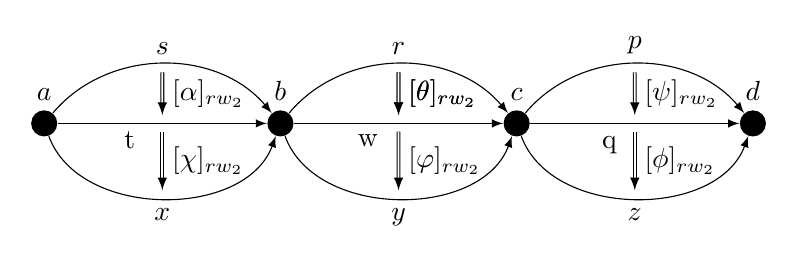
\begin{tikzpicture}[>=latex,
		every node/.style={auto},
		arrowstyle/.style={double,->,shorten <=3pt,shorten >=3pt},
		mydot/.style={circle,fill}]
		
		\coordinate[mydot,label=above:$a$](a)  at (0,0);
		\coordinate[mydot,label=above:$b$](b) at (3,0);
		\coordinate[mydot,label=above:$c$](c) at (6,0);
		\coordinate[mydot,label=above:$d$](d) at (9,0);
		\draw[->]   (a) to[bend left=50]  coordinate (s) node[]{$s$}          (b);
		\draw[->]   (a) to coordinate (t) node[label={[label distance=-1cm]43:t}] {}    (b);
		\draw[->]   (a) to[bend right=70]  coordinate (x) node[,swap]{$x$}          (b);
		\draw[->]   (b) to[bend left=50]  coordinate (r) node[]{$r$}          (c);
		\draw[->]   (b) to coordinate (w) node[label={[label distance=-1cm]40:w}] {}    (c);
		\draw[->]   (b) to[bend right=70]  coordinate (y) node[,swap]{$y$}          (c);
		\draw[->]   (c) to[bend left=50]  coordinate (p) node[]{$p$}          (d);
		\draw[->]   (c) to coordinate (q) node[label={[label distance=-1cm]50:q}] {}    (d);
		\draw[->]   (c) to[bend right=70]  coordinate (z) node[,swap]{$z$}          (d);
		
		\draw[arrowstyle] (s) to node[right]{[$\alpha]_{rw_{2}}$} (t);
		\draw[arrowstyle] (t) to node[right]{[$\chi]_{rw_{2}}$} (x);
		\draw[arrowstyle] (r) to node[right]{[$\theta]_{rw_{2}}$} (w);
		\draw[arrowstyle] (w) to node[right]{[$\varphi]_{rw_{2}}$} (y);
		\draw[arrowstyle] (r) to node[right]{[$\theta]_{rw_{2}}$} (w);
		\draw[arrowstyle] (p) to node[right]{[$\psi]_{rw_{2}}$} (q);
		\draw[arrowstyle] (q) to node[right]{[$\phi]_{rw_{2}}$} (z);
		\end{tikzpicture}	
		
	\end{center}
	
	In this diagram we represent $1$-arrows and $2$-arrows between these $1$-arrows. The fact that $2$-arrows are equivalence classes is represented by the brackets.
	
	Since we are working with a higher structures, some new properties should be checked. One of these properties is the fact that $2$-arrows can be composed horizontally\cite{leinster1}. In other words, given $1$-morphisms $s: a \rightarrow b$, $r: b \rightarrow c$, $t: a \rightarrow b$, $w: b \rightarrow c$ and 2-morphisms $[\alpha]_{rw_{2}}: s \rightarrow t$ and $[\theta]_{rw_{2}}: r \rightarrow w$, one should be able to define a horizontal composition $\circ_{h}$: $([\theta]_{rw_{2}} \circ_{h} [\alpha]_{rw_{2}}): r \circ s \rightarrow w \circ t$.
	
	Given $[\alpha]_{rw_{2}}: [s = \alpha_{1}, ..., \alpha_{n} = t]$ and $[\theta]_{rw_{2}}: [r = \theta_{1}, ...,\theta_{m} = w]$, then we define the horizontal composition $([\theta]_{rw_{2}} \circ_{h} [\alpha]_{rw_{2}})$ as the sequence $[\tau(s = \alpha_{1}, r = \theta_{1}), ..., \tau(\alpha_{n},\theta_{1}) ..., \tau(\alpha_{n} = t,\theta_{m} = w)]_{rw_{2}}$.
	
	We also need to verify the associative and identity law for $\circ_{h}$. Since we are working with a weak $2$-category, these laws should hold up to natural isomorphism \cite{leinster1}. To verify these laws, the idea is that every $2$-morphism of $[A_{rw_{2}}]$ is an isomorphism. To see that, remember that $rw$-equality is transitive, symmetric and reflexive. Therefore, if we have $[\theta]_{rw_{2}}$, we can think of the inverse $[\sigma(\theta)]_{rw_{2}}$. If we compose them, we have that  $[\theta]_{rw_{2}} \circ [\sigma(\theta)]_{rw_{2}} = [\theta \circ \sigma(\theta)]_{rw_{2}}$. Since we have in $LND_{EQ}-TRS_{2}$ that $(\theta \circ \sigma(\theta)) = \tau(\sigma(\theta),\theta)) \rhd_{tsr_{2}} \rho_{r}$, then $\theta \circ \sigma(\theta) =_{rw_{2}} \rho_{r}$ and thus, $[\theta \circ \sigma(\theta)]_{rw_{2}} = [\rho_{r}]_{rw_{2}}$. Analogously, one can prove that  $[\sigma(\theta) \circ \theta]_{rw_{2}} = [\rho_{w}]_{rw_{2}}$. Therefore, every $2$-morphism of $[A_{rw_{2}}]$ is an isomorphism. Since a natural transformation is a natural isomorphism iff every component is an isomorphism (as one can check in the \textbf{chapter 3}), we conclude that finding isomorphisms for the associative and identity laws is just a matter of finding the correct morphisms.
	
	For the associative law, we need to check that there is a natural isomorphism between $(([\psi]_{rw_{2}} \circ_{h} [\theta]_{rw_{2}}) \circ_{h} [\alpha]_{rw_{2}})$ and  $([\psi]_{rw_{2}} \circ_{h} ([\theta]_{rw_{2}} \circ_{h} [\alpha]_{rw_{2}}))$. To do this, by the definition of horizontal composition, a component of $(([\psi]_{rw_{2}} \circ_{h} [\theta]_{rw_{2}})$ is a term of the form $\tau(\alpha_{x}, \tau(\theta_{y}, \psi_{z}))$, with $x, y$, and $z$ being suitable natural numbers that respect the order of the horizontal composition. Analogously, the same component of  $([\psi]_{rw_{2}} \circ_{h} ([\theta]_{rw_{2}} \circ_{h} [\alpha]_{rw_{2}}))$ is just a suitable term  $\tau(\tau(\alpha_{x},\theta_{y}), \psi_{z})$. The isomorphism between these component is clearly established by the inverse $tt$ rule, i.e.,  $\tau(\alpha_{x}, \tau(\theta_{y}, \psi_{z})) =_{rw_{\sigma(tt)}} \tau(\tau(\alpha_{x},\theta_{y}), \psi_{z})$
	
	The identity laws use the same idea. We need to check that $([\alpha]_{rw_{2}} \circ_{h} [\rho_{\rho_{a}}]_{rw_{2}}) =  [\alpha]_{rw_{2}}$. To do that, we need to take components $(\rho_{\rho_{a}}, \alpha_{y})$ and $\alpha_{y}$ and establish their isomorphism: $(\rho_{\rho_{a}}, \alpha_{y}) =_{rw_{tlr}} \alpha_{y}$.
	
	The other natural isomorphism, i.e., the isomorphism between  $( [\rho_{\rho_{b}}]_{rw_{2}} \circ_{h} [\alpha]_{rw_{2}})$ and $[\alpha]_{rw_{2}}$ can be established in an analogous way, just using the rule $trr$ instead of $tlr$. Just for purpose of clarification, $\rho_{\rho_{a}}$ comes from the reflexive property of $rw$-equality. Since $\rho_{a}$ is the identity path, using the reflexivity we establish that $\rho_{a} =_{rw} \rho_{a}$, generating $\rho_{\rho_{a}}$.
	
	
	We call the associative morphism generated by $\sigma(tt)$ as $assoc$ (sometimes also called simply $a$), the morphism generate by $tlr$ as $l^{*}_{s}$ and the one generated by $trr$ as $r^{*}_{s}$. With the associative and identity isomorphisms established, we now need to check the \emph{interchange law}\cite{leinster1}. We need to check that:
	\begin{center}
		$([\varphi]_{rw_{2}} \circ [\theta]_{rw_{2}}) \circ_{h} ([\chi]_{rw_{2}} \circ [\alpha]_{rw_{2}}) = ([\varphi]_{rw_{2}} \circ_{h} [\chi]_{rw_{2}}) \circ ([\theta]_{rw_{2}} \circ_{h} [\alpha]_{rw_{2}})$
	\end{center}
	
	From  $(([\varphi]_{rw_{2}} \circ [\theta]_{rw_{2}}) \circ_{h} ([\chi]_{rw_{2}} \circ [\alpha]_{rw_{2}}))$, we have:
	
	\begin{center}
		$(([\varphi]_{rw_{2}} \circ [\theta]_{rw_{2}}) \circ_{h} ([\chi]_{rw_{2}} \circ [\alpha]_{rw_{2}})) =$
		
		$[\tau(\theta, \varphi)]_{rw_{2}} \circ_{h} [\tau(\alpha, \chi)]_{rw_{2}}=$
		
		$[\theta_{1}, ..., \theta_{n} = \varphi_{1}, ..., \varphi_{n'}]_{rw_{2}} \circ_{h} [(\alpha_{1}, ..., \alpha_{m} = \chi_{1}, ... \chi_{m'}]_{rw_{2}} = $
		
		$[\tau(\alpha_{1}, \theta_{1}),..., \tau(\alpha_{m} = \chi_{1}, \theta_{1}), ..., \tau(\chi_{n},\theta_{1}), ..., \tau(\chi_{n},\theta_{m'} = \varphi_{1}),..., \tau(\chi_{n},\varphi_{n'})]_{rw_{2}}$
	\end{center}
	
	From   $(([\varphi]_{rw_{2}} \circ_{h} [\chi]_{rw_{2}}) \circ ([\theta]_{rw_{2}} \circ_{h} [\alpha]_{rw_{2}})))$:
	
	\begin{center}
		$(([\varphi]_{rw_{2}} \circ_{h} [\chi]_{rw_{2}}) \circ ([\theta]_{rw_{2}} \circ_{h} [\alpha]_{rw_{2}}))(r \circ s) =$
		
		$([\tau(\chi_{1}, \varphi_{1}),...,\tau(\chi_{n},\varphi_{1}),...,\tau(\chi_{n},\varphi_{n'})]_{rw_{2}} \circ [\tau(\alpha_{1},\theta_{1}),...,\tau(\alpha_{m},\theta_{1}),...,\tau(\alpha_{m},\theta_{m'})]_{rw_{2}} = $
		
		$[\tau(\alpha_{1},\theta_{1}),...,\tau(\alpha_{m},\theta_{1}),...,\tau(\alpha_{m},\theta_{m'}),...,\tau(\chi_{1}, \varphi_{1}),...,\tau(\chi_{n},\varphi_{1}),...,\tau(\chi_{n},\varphi_{n'})]_{rw_{2}}$
		
	\end{center}
	
	If one looks closely, one can notice that this is a suitable to apply $cd_{2}$. Individually, every variable that appears in the sequence of transitivities follows the same expansion in both cases. The only difference is how the choices have been made. That way, if we construct $T$, as defined in Definition 4.6, one can check that $\tau(\alpha_{1}, \theta_{1}),..., \tau(\alpha_{m} = \chi_{1}, \theta_{1}), ..., \tau(\chi_{n},\theta_{1}), ..., \tau(\chi_{n},\theta_{m'} = \varphi_{1}),..., \tau(\chi_{n},\varphi_{n'}) \in T$ and $\tau(\alpha_{1},\theta_{1}),...,\tau(\alpha_{m},\theta_{1}),...,\tau(\alpha_{m},\theta_{m'}),...,\tau(\chi_{1}, \varphi_{1}),...,\tau(\chi_{n},\varphi_{1}),...,\tau(\chi_{n},\varphi_{n'}) \in T$  For that reason, we establish:
	\begin{center}
		$[\tau(\alpha_{1}, \theta_{1}),..., \tau(\alpha_{m} = \chi_{1}, \theta_{1}), ..., \tau(\chi_{n},\theta_{1}), ..., \tau(\chi_{n},\theta_{m'} = \varphi_{1}),..., \tau(\chi_{n},\varphi_{n'})]_{rw_{2}} =_{cd_{2}} [\tau(\alpha_{1},\theta_{1}),...,\tau(\alpha_{m},\theta_{1}),...,\tau(\alpha_{m},\theta_{m'}),...,\tau(\chi_{1}, \varphi_{1}),...,\tau(\chi_{n},\varphi_{1}),...,\tau(\chi_{n},\varphi_{n'})]_{rw_{2}}$. 
	\end{center}
	Since we are working with equivalence classes, this equality holds strictly.
	
	To end the proof, there is one more thing that we should verify. Since we are working with a weak structure, there is some laws that should hold. These laws are known as \emph{coherence laws}. In a weak $2$-category, the coherence laws are the following fact\cite{leinster1}:
	
	Given the following diagram of $1-morphisms$:
	
	\bigskip
	
	\begin{center}
		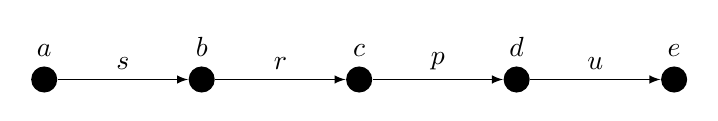
\begin{tikzpicture}[>=latex,
		every node/.style={auto},
		arrowstyle/.style={double,->,shorten <=3pt,shorten >=3pt},
		mydot/.style={circle,fill}]
		
		\coordinate[mydot,label=above:$a$](a)  at (0,0);
		\coordinate[mydot,label=above:$b$](b) at (2,0);
		\coordinate[mydot,label=above:$c$](c) at (4,0);
		\coordinate[mydot,label=above:$d$](d) at (6,0);
		\coordinate[mydot,label=above:$e$](e) at (8,0);
		
		\draw[->]   (a) to coordinate (s) node[] {$s$}    (b);
		\draw[->]   (b) to coordinate (r) node[] {$r$}    (c);
		\draw[->]   (c) to coordinate (p) node[] {$p$}    (d);
		\draw[->]   (d) to coordinate (u) node[] {$u$}    (e);
		
		
		\end{tikzpicture}
	\end{center}
	
	\bigskip
	
	The following diagrams should commute:
	
	\bigskip
	
	\begin{center}
		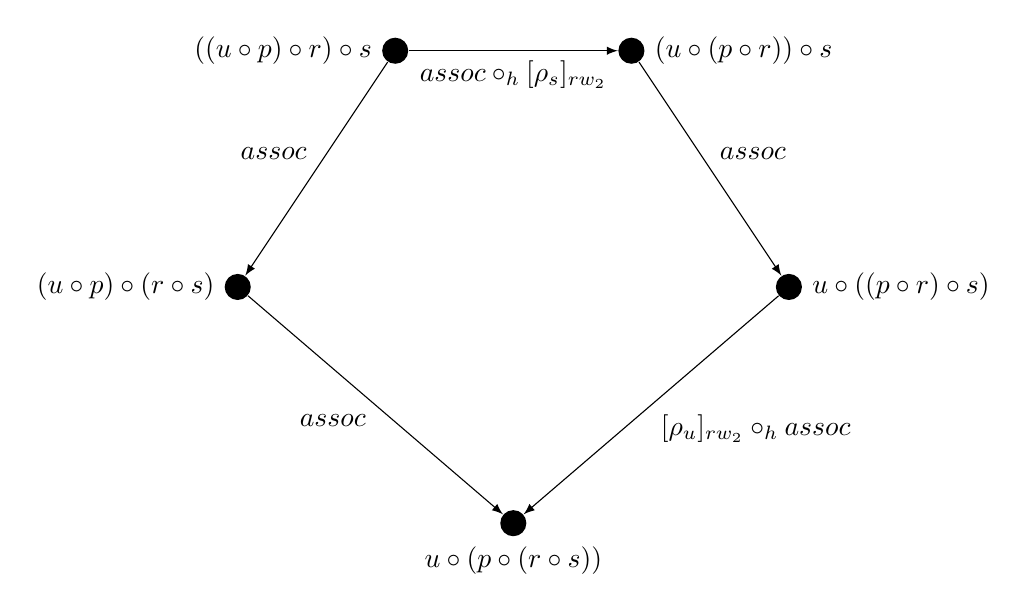
\begin{tikzpicture}[>=latex,
		every node/.style={auto},
		arrowstyle/.style={double,->,shorten <=3pt,shorten >=3pt},
		mydot/.style={circle,fill}]
		
		\coordinate[mydot,label=left:$((u\circ p) \circ r) \circ s$](a)  at (2,0);
		\coordinate[mydot,label=left:$(u \circ p) \circ (r \circ s)$](b) at (0,-3);
		\coordinate[mydot,label=right:$(u \circ(p \circ r)) \circ s$](c) at (5,0);
		\coordinate[mydot,label=right:$u \circ((p \circ r) \circ s) $](d) at (7,-3);
		\coordinate[mydot,label=below:$u \circ (p \circ (r \circ s))$](e) at (3.5,-6);
		
		\draw[->]   (a) to coordinate (s) node[,swap] {$assoc$}    (b);
		\draw[->]   (a) to coordinate (t) node[,swap] {$assoc \circ_{h} [\rho_{s}]_{rw_{2}}$}    (c);
		\draw[->]   (c) to coordinate (x) node[] {$assoc$}    (d);
		\draw[->]   (b) to coordinate (y) node[,swap] {$assoc$}    (e);
		\draw[->]   (d) to coordinate (z) node[] {$[\rho_{u}]_{rw_{2}} \circ_{h} assoc$}    (e);
		\end{tikzpicture}
		
		\bigskip
		
		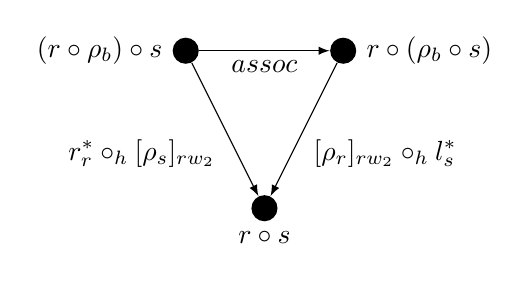
\begin{tikzpicture}[>=latex,
		every node/.style={auto},
		arrowstyle/.style={double,->,shorten <=3pt,shorten >=3pt},
		mydot/.style={circle,fill}]
		
		\coordinate[mydot,label=left:$(r \circ \rho_{b}) \circ s$](a)  at (0,0);
		\coordinate[mydot,label=right:$r \circ (\rho_{b} \circ s)$](b) at (2,0);
		\coordinate[mydot,label=below:$r \circ s$](c) at (1,-2);
		
		\draw[->]   (a) to coordinate (s) node[,swap] {$assoc$}    (b);
		\draw[->]   (a) to coordinate (t) node[,swap] {$r^{*}_{r} \circ_{h} [\rho_{s}]_{rw_{2}}$}    (c);
		\draw[->]   (b) to coordinate (x) node[] {$[\rho_{r}]_{rw_{2}} \circ_{h} l^{*}_{s}$}    (c);
		\end{tikzpicture}
	\end{center}
	
	\bigskip
	
	The proofs are straightforward. Remember that $assoc$ is just an application of $\sigma(tt)$, $r^{*}_{r}$ is an application of $trr$ and $l^{*}_{s}$ an application of $tlr$. First, let's start with $((u\circ p) \circ r) \circ s = \tau(s,\tau(r,\tau(p,u)))$ going to the right of the diagram:
	\begin{center}
		$(assoc \circ_{h} [\rho_{s}]_{rw_{2}})(\tau(s,\tau(r,\tau(p,u)))) = \tau(s,assoc(\tau(r,\tau(p,u)))) =$
		
		$\tau(s,\tau(\tau(r,p),u))$
		
		$assoc(\tau(s,\tau(\tau(r,p),u))) = \tau(\tau(s,\tau(r,p)),u)$
		
		$([\rho_{u}]_{rw_{2}} \circ_{h} assoc)(\tau(\tau(s,\tau(r,p)),u)) = \tau(assoc(\tau(s,\tau(r,p))), u) = $
		
		$\tau(\tau(\tau(s,r),p)), u) = u \circ (p \circ (r \circ s))$
	\end{center}
	
	Now, starting from the same $ \tau(s,\tau(r,\tau(p,u)))$ and going bottom left:
	
	\begin{center}
		$assoc(\tau(s,\tau(r,\tau(p,u)))) = \tau(\tau(s,r),\tau(p,u))$
		
		$assoc(\tau(\tau(s,r),\tau(p,u))) = \tau(\tau(\tau(s,r),p),u) = u \circ (p \circ (r \circ s))$
	\end{center}
	
	Therefore, the first diagram commutes. We now need to check the second one. Let's start from $((r \circ \rho_{b}) \circ s) = \tau(s,\tau(\rho_{b},r))$ and going to the right of the diagram:
	
	\begin{center}
		$assoc(\tau(s,\tau(\rho_{b},r))) = \tau(\tau(s,\rho_{b}),r)$
		
		$([\rho_{r}]_{rw_{2}} \circ_{h} l^{*}_{s})\tau(\tau(s,\rho_{b}),r) = \tau(l^{*}_{s}(\tau(s,\rho_{b})),r) = $
		
		$\tau(s,r) = r \circ s$
	\end{center}
	
	Now, starting from the same $\tau(s,\tau(\rho_{b},r))$ and going right bottom:
	
	\begin{center}
		$(r^{*}_{r} \circ_{h} [\rho_{s}]_{rw_{2}})\tau(s,\tau(\rho_{b},r)) = \tau(s,r^{*}_{r}(\tau(\rho_{b},r))) =$
		
		$\tau(s,r) = r \circ s$
	\end{center}
	
	Thus, the second diagram commutes. The coherence laws hold. We finally finish the proof that $[2-A_{rw}]$ is a weak $2$-category.
\end{proof}

We can also conclude that $[2-A_{rw}]$ has a weak $2$-groupoid structure. That is the case because we already know (from \emph{proposition 4.4}) that the groupoid laws are satisfied by $1$-morphisms up to the isomorphism of the next level, i.e., up to $rw$-equality and the $2$-morphisms, as we have just seen, are isomorphisms (that hold in a strict way, since the second level is using classes of equivalence).  With that, we showed that computational paths induces a $2$-weak groupoid. If one compares this groupoid with the one obtained by the homotopy interpretation, this $2$-weak category is similar to the fundamental weak $2$-groupoid of a space $S$, denoted by $\Pi_{2} S$ (that $\Pi_{2} S$ forms a weak $2$-category can be seen in \cite{Tom}).

Since we could induce a weak $2$-categorical structure using computational paths, would be possible to induce even higher structures? The answer is $yes$, since we have infinite levels of $rw$-rules established by infinite $LND_{EQ}-TRS_{n}$ systems. For example, we could add a new level $A_{3rw}(\theta,\alpha)$. where $\theta$ and $\alpha$ are $2$-morphisms. We would have a structure with $3$ levels and we could try to prove that this structure is a weak $3$-category. The problem is, as one could see in the proof of \emph{proposition 4.5}, working with higher structures can be difficult. A weak $3$-weak category has more types of compositions than the $2$-weak one, since we have an additional level. Moreover, since it is weak, there are coherence laws that must be checked. For a $3$-weak category, these laws are much more complicated than the ones for $2$-weak categories. For that reason, we will leave the study of higher structures induced by computational paths with more than $2$ levels for the future, since it is still work in progress. In fact, our aim is to prove, in a future work, that computational path induces a weak category with infinite levels, known as weak $\omega$-category. In fact, we want to show that this weak infinite category forms a weak $\omega$-groupoid. We believe that it is possible to achieve these results, since it was proved by\cite{lumsdaine1,Benno} that the identity type induces such structure. Given the connection between computational paths and terms of identity types, we should be able to prove that computational paths also induces a weak $\omega$-groupoid.

\section{Uniqueness of Identity Proofs}

One of the main results that arises from the groupoid interpretation of\cite{hofmann2} is that it refutes the uniqueness of identity proofs, also known as $UIP$.\cite{hofmann2} defines UIP as the following property:

\begin{mydefi}
	
	Let $a$ and $b$ be objects of a type $A$. $UIP$ is the following property: given any proofs $p$ and $q$ of proposition $a$ equals to $b$, then there is always another proof establishing the equality of $p$ and $q$.
	
\end{mydefi}

In terms of computational paths, $UIP$ asks if, for every pair of objects $t$ and $s$ between $a$ and $b$ of a type $A$, there is an $rw$-equality $t =_{rw_{\theta}} s$. To better see this situation, a concrete example is given by\cite{Ruy1}:

\begin{example}
	Consider the term $(\lambda x.(\lambda y.yx)(\lambda w.zw))v$. We want to reduce this term to the term $zv$. To achieve this goal, we can follow 3 different paths:
	
	\begin{itemize}
		\item $(\lambda x.(\lambda y.yx)(\lambda w.zw))v$ $\rhd_{\eta}$ $(\lambda x.(\lambda y.yx)z)v$ $\rhd_{\beta}$ $(\lambda y.yv)z$ $\rhd_{\beta}$ $zv$.
		
		\item $(\lambda x.(\lambda y.yx)(\lambda w.zw))v$ $\rhd_{\beta}$ $(\lambda x.(\lambda w.zw)x)v$ $\rhd_{\eta}$ $(\lambda x.zx)v$ $\rhd_{\beta}$ $zv$.
		
		\item $(\lambda x.(\lambda y.yx)(\lambda w.zw))v$ $\rhd_{\beta}$ $(\lambda x.(\lambda w.zw)x)v$ $\rhd_{\beta}$ $(\lambda w.zw)v$ $\rhd_{\eta}$ $zv$.
		
	\end{itemize}
	
\end{example}

Thus, if $UIP$ holds, those 3 paths are just different ways of expressing the same thing. In other words, it would be possible to find $rw$-equalities establishing equalities between them.

The objective of this section is to show that, similarly to the traditional approach for the identity type, our path-based one also refutes $UIP$. Given a type $A$, by the definition of $UIP$, one can conceive a type $UIP(A)$ that is inhabited iff for any terms $a,b : A$ and paths $a =_{s} b$ and $a =_{t} b$, then $s =_{rw} t$. 

As stated by\cite{hofmann2}, if $UIP$ holds, then every type $A$ is a trivial groupoid structure in which there is only one morphism between every pair of objects. To show that $UIP$ is false, one only needs to construct an $A$ such that there is more than one morphism between a pair of objects (i.e., there is at least one pair of objects $a,b : A$ and a pair of paths $s$ and $t$ between them such that $s that $ $s \neq_{rw} t$). To achieve that, we can take advantage of our previous example, and consider  $(\lambda x.(\lambda y.yx)(\lambda w.zw))v : A$. Therefore \cite{Art3,Ruy1}:

\begin{theorem}
	The type $UIP$ is empty.
\end{theorem}

\begin{proof}
	We construct $A_{rw}$:
	
	
	\begin{center}
		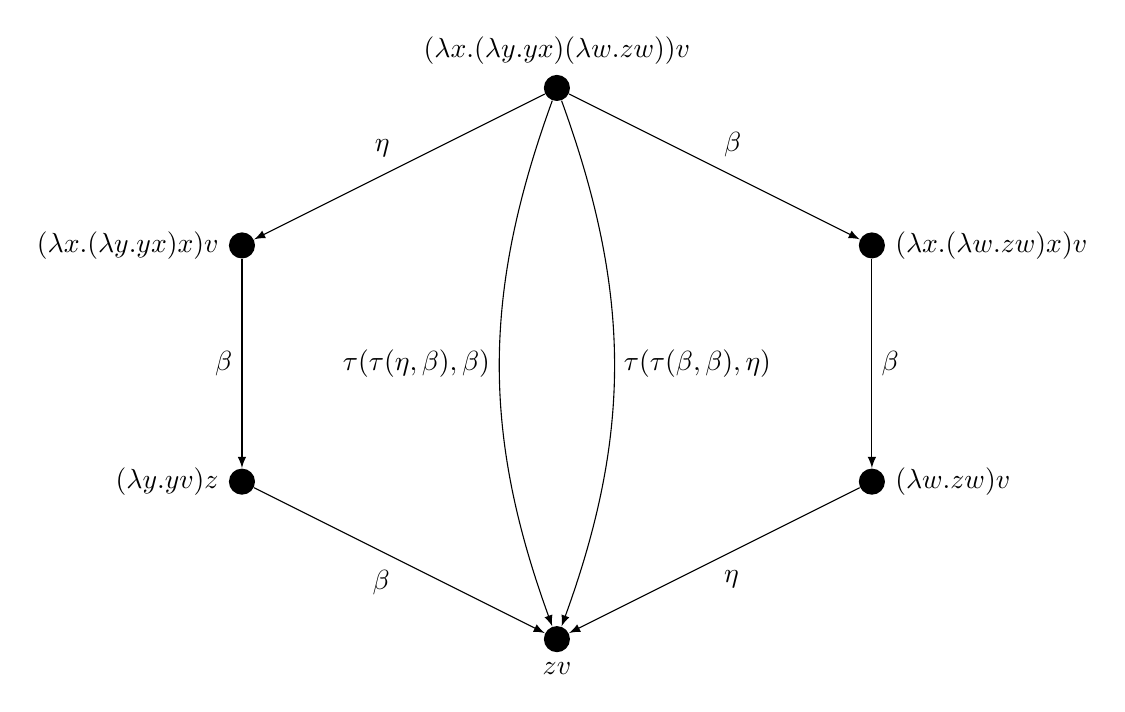
\begin{tikzpicture}[>=latex,
		every node/.style={auto},
		arrowstyle/.style={double,->,shorten <=3pt,shorten >=3pt},
		mydot/.style={circle,fill}]
		
		\coordinate[mydot,label=above:$(\lambda x.(\lambda y.yx)(\lambda w.zw))v$](a)  at (5,0);
		\coordinate[mydot,label=left:$(\lambda x.(\lambda y.yx)x)v$](b) at (1,-2);
		\coordinate[mydot,label=left:$(\lambda y.yv)z$](c) at (1,-5);
		\coordinate[mydot,label=below:$zv$](d) at (5,-7);
		\coordinate[mydot,label=right:$(\lambda x.(\lambda w.zw)x)v$](e) at (9,-2);
		\coordinate[mydot,label=right:$(\lambda w.zw)v$](f) at (9,-5);
		
		
		\draw[->]   (a) to coordinate (eta1) node[,swap] {$\eta$}    (b);
		\draw[->]   (b) to coordinate (beta1) node[,swap] {$\beta$}    (c);
		\draw[->]   (c) to coordinate (beta2) node[,swap] {$\beta$}    (d);
		%\draw[->]   (b) to coordinate (y) node[,swap] {$assoc$}    (e);
		\draw[->]   (a) to[bend right = 20] coordinate (z) node[,swap] {$\tau(\tau(\eta,\beta),\beta)$}    (d);
		\draw[->]   (a) to[bend left = 20] coordinate (z) node[] {$\tau(\tau(\beta,\beta),\eta)$}    (d);
		\draw[->]   (a) to coordinate (beta3) node[] {$\beta$}    (e);
		\draw[->]   (e) to coordinate (beta4) node[] {$\beta$}    (f);
		\draw[->]   (f) to coordinate (beta4) node[] {$\eta$}    (d);
		\end{tikzpicture}
		
	\end{center}
	
	\bigskip
	
	As depicted above, there are (at least) two possible paths between $(\lambda x.(\lambda y.yx)(\lambda w.zw))v$ and $zv$. The first path is given by $\tau(\tau(\eta,\beta),\beta)$ and the second by $\tau(\tau(\beta,\beta),\eta)$. Moreover, looking at all $rw$-rules (check \textbf{definition 4.18}), there is no rule that establishes the $rw$-equality between these two paths. That way, $A_{rw} $ is not a trivial groupoid and thus, $UIP$ is empty.
\end{proof} 

With that, we conclude that our approach based on computational paths refutes the uniqueness of identity proofs.

\section{Conclusion}

Inspired by a recent discovery that the propositional equality between terms can be interpreted as the type of homotopy paths, we have revisited the formulation of the intensional identity type, proposing a approach based on an entity known as {\em computational path}. We have proposed that a computational path $a =_{s} b : A$ gives grounds to building a term $s(a,b)$ of the identity type, i.e., $s(a,b) : Id_{A}(a,b)$, and is formed by a composition of basic rewrites, each with their identifiers taken as constants. We have also developed our approach, showing how the path-based identity type can be rather straightforwardly used in deductions. In particular, we have shown the simplicity of our elimination rule, demonstrating that it is based on path constructions, which are built from applications of simple axioms of the equality for type theory. To make our point even clearer, we have exposed three path-based constructions. More specifically, constructions that prove the transitivity, reflexivity and symmetry of the propositional equality. We have also argued that, for these constructions, the process of finding the reason that allows for building the desired term was simple and straightforward in our approach. At the same time, in the traditional (or pathless) approach, this is not entirely true, since finding the correct reason was a cumbersome process.

After establishing the foundations of our approach, we analyzed one important structure that the traditional identity type induces: the algebraic structure known as groupoid. Our objective was to show that our approach is on a par with the pathless one, i.e., our path-based identity also induces a groupoid structure. To prove that, we have shown that the axioms of equality generate redundancies, which are resolved by paths between paths. We mentioned that there already exists a system called $LND_{EQ}-TRS$ that maps and resolves these redundancies.  We have gone further, proposing the existence of a higher $LND_{EQ}-TRS_{2}$ which resolves redundancies generated by the $LND_{EQ}-TRS$ system. Using  $LND_{EQ}-TRS$, we have proved that a computational path is capable of inducing a weak groupoid structure. Using the higher rewriting system, we have induced a structure known as weak $2$-groupoid. With that, we believe we have opened the way, in a future work, for a possible proof establishing that computational paths induces a weak $\omega$-groupoid.

We have also shown that, using our groupoid of computational paths, it is possible to refute the principle of uniqueness of identity proofs for the path-based approach. This result ties in with the one obtained by \cite{hofmann2} for the traditional identity type.